\documentclass[11pt]{article}
\usepackage[T1]{fontenc}
\usepackage{lmodern}
\usepackage{microtype}
\usepackage[a4paper,margin=27mm,headheight=14pt]{geometry}
\usepackage{amsmath,amssymb,amsthm,mathtools}
\usepackage{booktabs,longtable,array,graphicx}
\usepackage{xcolor}
\usepackage{enumitem}
\usepackage{fancyhdr}
\usepackage{url}
\usepackage[breaklinks]{hyperref}
\definecolor{ink}{HTML}{18354D}
\definecolor{accent}{HTML}{126A7A}
\definecolor{wash}{HTML}{EFF5F7}
\hypersetup{colorlinks=true,linkcolor=ink,citecolor=accent,urlcolor=accent,
  pdftitle={Saturating Raw Tietze Eliminations and Indexing Certified Interval Orbits},
  pdfauthor={Research continuation prepared for Vladimir Reshetnikov}}
\urlstyle{same}
\setlength{\emergencystretch}{2em}
\setlist{itemsep=3pt,topsep=5pt}
\newtheorem{theorem}{Theorem}[section]
\newtheorem{lemma}[theorem]{Lemma}
\newtheorem{proposition}[theorem]{Proposition}
\newtheorem{corollary}[theorem]{Corollary}
\theoremstyle{definition}
\newtheorem{definition}[theorem]{Definition}
\newtheorem{example}[theorem]{Example}
\theoremstyle{remark}
\newtheorem{remark}[theorem]{Remark}
\DeclareMathOperator{\supp}{supp}
\DeclareMathOperator{\cl}{cl}
\DeclareMathOperator{\per}{per}
\newcommand{\QPoly}{\operatorname{QP}}
\pagestyle{fancy}
\fancyhf{}
\fancyhead[L]{\small\color{ink}Compiled certificates for unknot recognition}
\fancyhead[R]{\small Research continuation}
\fancyfoot[C]{\thepage}
\renewcommand{\headrulewidth}{0.3pt}
\title{\color{ink}\bfseries Saturating Raw Tietze Eliminations\\[3pt]
  and Indexing Certified Interval Orbits}
\author{Research continuation prepared for Vladimir Reshetnikov\\
  \small ProveIt / Topology / UnknotRecognition}
\date{9 October 2026 (UTC)\\
  \small Source baseline: \texttt{fdeb5b1a20b84b93cb150e0232031837bb7d30cb}}

\begin{document}
\maketitle
\begin{abstract}
We develop two exact improvements to the maintained unknot-recognition
project. First, we prove that every completed epoch of raw singleton
Tietze eliminations can be flattened into one acyclic batch of definitions
from its original relator slots. A nonnegative occurrence matrix and a
unique-perfect-matching argument account for the required reassignment of
donors. Consequently, reduction to a prescribed survivor alphabet is
equivalent to a source Horn-closure query. After source metadata preparation,
one query uses $O(r+m+I)$ structural operations, and exhaustive rank-one
discovery uses $O(r(r+m+I))$, where $r$ is the generator count, $m$ the
number of source relator slots, and $I$ their total distinct-support
incidence. The resulting batch has polynomial grammar size independently
of the number of raw phases it replaces. An optional production hook uses
the existing independent certificate verifier.

Second, we compile a checked Agol--Hass--Thurston orbit trace into reusable
point-to-component queries. The component key is the least original point
of the orbit, so it is independent of the valid reduction trace. Binary
arithmetic replaces repeated orbit searches; component representatives
remain compressed even when their number is enormous. In fact, the entire
set of minimum representatives is a union of at most $g$ ordinary intervals,
where $g$ is the trace's static-gap count, giving canonical rank and selection
in $O(B\log(g+2))$ bit operations after preparation, where $B$ bounds
coordinate and counter bit lengths. We give complete
proofs, adversarial examples, source-bound tests, and paired measurements
with controls. The results improve precisely defined algebraic and
geometric operations. They do not bound normalization between raw epochs,
normal-surface discovery, or hierarchy search, and therefore do not
establish general quasi-polynomial unknot recognition.
\end{abstract}

\begin{center}
\fcolorbox{accent}{wash}{\parbox{0.92\linewidth}{\small
\textbf{Scope of the result.} The new completeness theorem concerns
\emph{all orders of raw singleton elimination from a fixed presentation}.
The new geometric interface concerns \emph{many queries on one certified
interval relation}. The general recognition pipeline retains its previous
worst-case guarantee. Successful knot certificates are independently
replayed; exhaustion of either local query class is inconclusive about knot type.}}
\end{center}
\tableofcontents
\newpage

\section{Research objective and source audit}
\label{sec:background}

The project already has an exact recognition pipeline with several
independent positive certificates and negative obstructions. The relevant
question is which repeated operations can be replaced by a provably smaller
computation, while preserving the source binding and the certificate
checker. This continuation makes two such replacements. It also identifies
the transformations that the new theorems do not cover, so the next
complexity question is explicit.

\subsection{A pinned and executable baseline}

All implementation comparisons use commit
\texttt{fdeb5b1a20b84b93cb150e0232031837bb7d30cb}
of \texttt{VladimirReshetnikov/ProveIt}, observed at the start of this work.
The repository's upstream branch may continue to move. A manifest records
the exact Git blob identifiers of the retrieved source files, and the
benchmark outputs record SHA256 hashes of the modules actually loaded.
The archive contains a reference snapshot for the paired group comparisons
and the additional reference modules required by the maintained test suite.

The immediately relevant maintained components are:
\begin{itemize}
\item \path{fastunknot/compressed_words.py}: exact shared word grammars,
  compressed equality, slicing, inversion, and free reduction;
\item \path{elimination_batch.py} and its independent verifiers:
  simultaneous acyclic singleton definitions, with source relator slots
  retained throughout replay;
\item \path{compressed_search.py}: the optional group search, including
  normalization boundaries, Whitehead transformations, overlap moves,
  and arithmetic terminal tests;
\item \path{interval_orbits.py} and \path{interval_orbit_verify.py}:
  binary interval-orbit counting and independent local-trace replay;
\item the native normal-surface geometry and weighted-component modules,
  which interpret interval orbits as components of a supplied surface.
\end{itemize}
The associated synthesis sections already discuss raw acyclic batches,
incremental reachability, memoized word frontiers, weighted components,
and normal-surface certificates~\cite{repo}. The present work does not
reintroduce those operations as new results. The substantive additions are
the completeness characterization of an entire raw epoch, its source
closure producer, and the reusable component-query interface.

\subsection{What the quasi-polynomial target currently means}

For input size $n$, quasi-polynomial time means
$\exp((\log n)^{O(1)})$. The more specific target
$n^{O(\log n)}=\exp(O((\log n)^2))$ is stronger than
$\exp(O((\log n)^3))$. These bounds should not be interchanged.

Lackenby's publicly available March 2021 handout states the latter bound,
$2^{O((\log n)^3)}$, for a diagram with $n$ crossings. Its hierarchy
outline combines a quadratic bound on its surface-complexity parameter $g$ with
depth $O((\log n)^2)$~\cite{lackenby-talk}. His July 2026 preprint provides
substantial detailed hierarchy machinery and proves an
$\mathrm{NP}\cap\mathrm{coNP}$ result for essential boundary patterns.
However, its Section 9 explicitly leaves the costs of individual steps
insufficiently specified, and bounds their number in terms of two
parameters by $L(g+1)^L$~\cite{lackenby-2026}. We have not identified a
complete public specification of the announced quasi-polynomial algorithm
that can simply be translated into this codebase.

This distinction does not diminish the role of the published compressed
primitives. Agol--Hass--Thurston (AHT) already give polynomial orbit counting
in the pairing count and logarithmic interval length, and a weighted
version for topology of a supplied normal surface~\cite{aht}. Lackenby's
2026 curve algorithms similarly give polynomial dependence on surface
triangulation size and logarithmic curve weights~\cite{lackenby-curves}.
The remaining difficulty includes producing appropriate objects and
controlling how many successive objects or search states arise.

\subsection{Two distinct sources of repeated work}

The algebraic computation repeatedly substitutes generator definitions
into shared grammars. A local batch can be small relative to the grammar
at its start, while multiplying a coarse bound across many phases gives
an exponential factor in phase depth. We ask whether the intermediate
phases are needed at all when no cancellation or other transformation
occurs between them. The answer is no: complete raw reachability is a
query on the original source support.

The geometric computation has a different redundancy. After certifying
one interval equivalence relation, it can be asked repeatedly whether
marked points lie on the same component. The existing general membership
test creates an additional identification and recounts orbits. We instead
retain the point transport implicit in one checked trace. This removes
repeated schedule discovery, without changing the relation or replacing
binary coordinates by explicit points.

Both improvements distinguish discovery from verification. The group
producer returns an established certificate format that the old verifier
already understands. The orbit index first checks its entire source trace,
then answers queries using an audited transport implementation. The second
interface does not claim to produce a separate independently checkable
proof for every point answer.

\section{Preliminaries and cost conventions}
\label{sec:preliminaries}

\subsection{Presentations and raw words}

Let $X$ be a finite set of positive generator names. A raw word is a finite
sequence in $X^{\pm1}$. Its \emph{absolute occurrence count} of $x$ counts
both $x$ and $x^{-1}$, while its exponent sum subtracts negative from
positive occurrences. Its support is the set of generator names occurring
at least once. Raw word equality, equality after free reduction, and
equality in a presented group are three different relations.

Relators are stored in numbered slots. Empty words and repeated roots may
occur. Consuming a donor empties that slot; it does not renumber the other
slots. A source for a new raw epoch may be obtained after a previously
verified presentation transformation. Thus the theorem applies to general
current source words, and is not limited to the length-four Wirtinger
relators of the initial knot diagram.

The native arena represents words by an acyclic straight-line grammar with
letter leaves and binary concatenation nodes. Children are allocated before
parents. Multiple roots share subgraphs, and repeated uses of a child are
repeated occurrences in the expanded word. Exact compressed free-group
operations are established polynomial primitives~\cite{schleimer}; they
are not probabilistic hash tests. The saturation query itself requires
only raw presence and repetition information.

\subsection{Parameters that are kept separate}

For one source presentation write
\[
 r=|X|,\qquad m=\text{number of relator slots},\qquad
 I=\sum_{j=1}^{m}|\supp(R_j)|,
\]
and let $M$ and $H$ be its reachable grammar size and height. The term $m$
must remain in cost bounds even if many slots are empty or share one root.
On a fresh compact source grammar, $H\le M$ and the maximum expanded-word
length has $O(M+1)$ bits. Generator names and node identifiers have their
own encoded lengths; dense local renaming handles large names without
allocating arrays up to the largest name.

Structural-operation estimates use ordinary random-access arrays and
indices. Python's dictionary accounting is stated where relevant. For a
strict deterministic bit bound, label sorting and array indices can replace
hash lookup, or its worst-case polynomial overhead can be charged. None of
the decisions depends on random hashing. The maintained arena may retain
an alphabet and caches from earlier search states. Its historical storage
and mask widths must be charged to that history, rather than silently
identified with the current rank or reachable subgrammar.

For interval systems, $N$ is the represented point count, $k$ the pairing
count, and $B$ the maximum bit length of coordinates and accumulated
counters. A trace has $E$ events. A claim polynomial in $B$ is very
different from a loop with $N$ iterations. Likewise, the number of
components may require only $B$ bits while an explicit component list is
infeasible. The algorithms below never require that list.

\section{Raw singleton epochs are a source closure problem}
\label{sec:raw-epoch-theorem}

The previous local analysis bounds one acyclic singleton batch polynomially
in its current grammar, and gives an exponential-in-depth bound for a succession
of batches. There is a stronger algorithmic alternative for an entire epoch
in which the only word transformations are raw singleton substitutions.
Such an epoch can be discovered on its immutable source incidence data and
compiled as one batch. The essential new statement is the equivalence with
\emph{every possible sequential raw elimination order}. Computing the least
closure of a family of implications is standard; matching acyclicity and
unique perfect matchings are standard as well~\cite{kozen,golumbic,dowling}.

\subsection{Precisely which epochs are covered}

Let $X$ be a finite set of positive generator labels, and let
$(R_1,\ldots,R_m)$ be a list of raw words in $X^{\pm1}$ represented by one
shared straight-line grammar. Empty and repeated slots are retained. Fix a
survivor set $S\subseteq X$, and put $E=X\setminus S$.

A raw singleton step chooses a previously unconsumed original slot $d$
whose current word is $U x^\epsilon V$, where $\epsilon\in\{1,-1\}$ and
the absolute letter $x$ occurs exactly once. It sets
\[
 x\longmapsto (VU)^{-\epsilon},
\]
substitutes this word and its formal inverse into every remaining slot,
and consumes slot $d$. Every substitution is performed on raw words:
there is no free reduction, cyclic reduction, proper-power root extraction,
Whitehead transformation, or relator multiplication between steps.
An acyclic raw batch can be linearized in dependency order, so is included.
The epoch succeeds for $S$ if it eliminates exactly $E$.

The frozen source itself may be the result of an already verified prefix
containing other moves. It is the transformations \emph{inside} the epoch
that are restricted. In particular, this theorem can be applied afresh at
each normalized presentation boundary. It does not combine the different
boundaries into one bounded-cost search.

For each source row $R_j$ and each generator $x$ occurring exactly once in
its raw spelling, form the implication
\[
 \operatorname{supp}(R_j)\setminus\{x\}\ \Longrightarrow\ x,
 \tag{H}\label{eq:raw-horn-rule}
\]
where support ignores signs but counts distinct labels. Let
$\operatorname{cl}(S)$ be the least set containing $S$ and closed under
these implications. Multiplicity one is essential: a zero exponent sum is
not absence, and a nonzero exponent sum of magnitude one does not imply a
unique raw occurrence.

\begin{theorem}[Complete source criterion for raw singleton reduction]
\label{thm:raw-closure-equivalence}
The following are equivalent:
\begin{enumerate}
\item Some raw singleton epoch reduces the frozen source to the survivor
      alphabet $S$.
\item Some acyclic singleton batch formed directly from original source
      slots eliminates $E$.
\item $\operatorname{cl}(S)=X$.
\end{enumerate}
If an epoch uses a specified donor-slot set $D$, with $|D|=|E|$, then it can
be flattened using exactly the same source slots $D$, after possibly
reassigning their eliminated generators. The flattened batch and that
epoch induce the same homomorphism $F(X)\to F(S)$ as free-group elements.
Their unreduced output strings need not agree.
\end{theorem}

The last assertion requires the same donor set. A generic closure search
over all source rows may select a different donor set from a previous
producer. Its resulting presentation is still Tietze equivalent to the
source, but its word images are not asserted equal to those of the previous
producer in $F(S)$. No equality of tied witnesses, subsequent search paths,
or finite-budget recognition outcomes is implied.

\subsection{The positive pivot lemma}

For a nonnegative integral square matrix $A$, write $\operatorname{per}(A)$
for its permanent, with permanent one for the empty matrix. Equivalently,
replace entry $a_{ij}$ by that many separately labelled parallel edges in a
bipartite graph; the permanent counts its edge-labelled perfect matchings.
The permanent is used only in the proof, not computed by the algorithm.

\begin{lemma}[Reversing a successful unit pivot]
\label{lem:positive-pivot}
Suppose $a_{dc}=1$. Delete row $d$ and column $c$ and set
\[
 b_{ij}=a_{ij}+a_{ic}a_{dj}\qquad(i\ne d,\ j\ne c).
\]
If $\operatorname{per}(B)=1$, then $\operatorname{per}(A)=1$.
\end{lemma}

\begin{proof}
Tag each edge counted by $b_{ij}$ either as an original direct edge from
$i$ to $j$, or as an ordered pair of original edges from $i$ to $c$ and
from $d$ to $j$. Consider the unique tagged perfect matching of $B$.
It contains at most one pair-created edge. Indeed, if it contained
pair-created edges $(i,j)$ and $(k,\ell)$, their source rows and destination
columns would be distinct. Exchanging the destination factors would give
pair-created edges $(i,\ell)$ and $(k,j)$ and a second tagged perfect
matching, a contradiction.

If it contains no pair-created edge, adjoin the unique edge $(d,c)$.
If it contains one, replace that edge by its two original component edges.
Either operation constructs a perfect matching of $A$.

Conversely, each perfect matching of $A$ maps injectively to a tagged
perfect matching of $B$. If it uses $(d,c)$, delete that edge. Otherwise
there is a unique row $i$ matched to $c$ and a unique column $j$ matched
from $d$; replace those two edges by the corresponding pair-created edge
$(i,j)$. All remaining edges are tagged direct. The number of pair-created
edges distinguishes the two cases, and their tags recover all original
occurrence choices. Thus $A$ has at most as many perfect matchings as
$B$. It has at least one by the preceding construction, proving the lemma.
\end{proof}

The converse of the lemma for an arbitrarily chosen pivot is false. For
example
\[
 A=\begin{pmatrix}1&1&1\\1&0&1\\1&0&0\end{pmatrix}
 \quad\hbox{has permanent }1,
\]
but pivoting its upper-left entry gives
$\left(\begin{smallmatrix}1&2\\1&1\end{smallmatrix}\right)$, whose permanent
is three. A poor raw elimination order can become stuck even when another
order would finish. The source closure algorithm avoids this order dependence.

\subsection{Flattening proof}

For a completed epoch, let $D$ be its consumed original slots and $E$ its
eliminated generators. Form the square source occurrence matrix
\[
 A_{jx}=\#\{\text{occurrences of }x\text{ or }x^{-1}\text{ in }R_j\},
 \qquad j\in D,\quad x\in E.
\]
At any stage restrict to the still-unconsumed rows of $D$ and still-live
columns of $E$. A raw singleton step has pivot one, and its new occurrence
matrix is exactly the positive pivot in Lemma~\ref{lem:positive-pivot}.
Deleting the unique pivot letter leaves $a_{dy}$ occurrences of every other
letter $y$ in its defining image. Each of the $a_{ix}$ occurrences in
another row contributes one such image. Inversion changes signs and order,
but not absolute occurrence counts. No cancellation subtracts occurrences.

The final matrix is empty. Applying the lemma backwards through every step
gives $\operatorname{per}(A)=1$. Let its unique perfect matching assign
source donor $R_{d(x)}$ to $x$. Every matched occurrence has multiplicity
one. Direct an edge $x\to y$ when $y\ne x$, $y\in E$, and $y$ appears in
$R_{d(x)}$. A directed cycle would allow cyclic exchange of the matched
columns and create a second perfect matching. Hence this definition graph
is acyclic. Solving the matched source equations in dependency order gives
a single acyclic batch eliminating $E$.

For the equality assertion, let $\phi:F(X)\to F(S)$ be the homomorphism
computed by the original epoch. A consumed equation becomes the identity
when it is eliminated, and stays the identity under subsequent
homomorphisms. Therefore $\phi(R_j)=1$ for every $j\in D$, and $\phi$ fixes
$S$. The acyclic matching gives a unique $F(S)$-valued solution to these
same equations with the values on $S$ fixed: determine each generator in
dependency order. Its homomorphism $\psi$ must consequently equal $\phi$.
In particular, freely reduced residual source words agree. This uniqueness
argument is in a free group, not in the monoid of unreduced signed strings.

For a concrete difference in raw spelling, take the two donor equations
\[
 R_1=xayb,\qquad R_2=xc,
\]
with $a,b,c$ surviving. Eliminating $x$ first from $R_1$, then $y$ from
the substituted $R_2$, sends $x$ to
$b^{-1}bc^{-1}aa^{-1}$ as a raw word. The source matching assigns $R_2$ to
$x$ and $R_1$ to $y$, and sends $x$ directly to $c^{-1}$. Both maps agree
in $F(a,b,c)$.

To finish Theorem~\ref{thm:raw-closure-equivalence}, an acyclic source
definition order is a sequence of productive applications of
\eqref{eq:raw-horn-rule}, so the closure contains every generator.
Conversely, record one source row whenever closure first adds a generator.
Its other support labels were already known, so the resulting definitions
are acyclic. A row cannot be used twice: after its first productive firing,
every member of its support is known. These distinct source rows therefore
give a valid acyclic Tietze batch. This proves all directions.

\subsection{Exact discovery without constructing intermediate words}

The implementation uses the maintained word arena's immutable presence and
repetition masks. At a concatenation $UV$ they satisfy
\[
 P_{UV}=P_U\cup P_V,\qquad
 Q_{UV}=Q_U\cup Q_V\cup(P_U\cap P_V).
\]
Consequently $P_R\setminus Q_R$ is precisely the set of raw singleton
generators. Two uses of the same child grammar still count twice. These
summaries never infer cancellation from exponent sums or from equality of
oppositely signed words.

From the summaries, build a sparse generator-to-source-slot incidence
index. For each row retain its number of currently unknown distinct
generators and the xor of their dense local indices. When the number is
one, the xor identifies the remaining generator. The row can fire exactly
when that generator is in its original singleton set. A queue processes
newly enabled rows. On learning a generator, decrement the unknown counts
and update the xors in its incident rows. A row can pass from two unknown
generators to one only once, so it enters the queue at most once; a queued
row can become stale by falling to zero before it is visited.

The invariant is that the counters and xors describe exactly the unknown
members of every row. Every firing is permitted by the implication rule.
When no row can fire, the known set is closed. By monotonicity it is the
least closed superset of the seeds. No word image, substring, inverse, or
new grammar node is created by this discovery pass.

There is an exact early failure condition for all singleton seeds. If
$r=|X|>1$ and no source row has support size at most two and at least one
raw singleton generator, then no singleton seed admits a first productive
firing. All singleton closures are trivial. This is a proof about this
algebraic query; it is not a nontrivial-knot test.

Let $I=\sum_j|\operatorname{supp}(R_j)|$. Once source metadata is available,
one closure uses $O(r+m+I)$ structural operations and $O(r+m+I)$ working
entries. The counters and local xors have $O(\log(r+1))$ bits. Trying all
$r$ one-element seeds therefore takes
\[
 O\bigl(r(r+m+I)\bigr)
\]
such operations, plus source summarization. This is expected dictionary
operation accounting for the Python implementation; label and identifier
bit costs must be charged separately. Persistent arena masks may use the
historical alphabet width rather than the current live rank. That existing
memory cost is not hidden in the sparse source index bound.

More generally, the fixed-$k$-survivor query can enumerate all
$\binom rk$ seed sets, for $0\le k\le r$, with total closure cost
\[
 O\!\left(\binom rk(r+m+I)\right).
\]
This also decides reducibility to \emph{at most} $k$ survivors: a smaller
successful seed set extends to size $k$, and closure is monotone. For
$k\ge r$ the answer is immediate by the empty epoch; $k=0$ is the single
empty-seed query. For $k<r$, absence of every source row with support at
most $k+1$ and a raw singleton similarly proves that no size-$k$ seed set
can make a first productive firing. Only the $k=1$ early guard is used in
the delivered planner.

On a freshly renumbered compact source of encoded length $n_0$, the
parameters $r,m,M$ are $O(n_0)$ and $I\le mr=O(n_0^2)$. The one-seed
enumeration thus uses $O(n_0^3)$ structural operations after preparation.
Computing presence/repetition bit vectors, enumerating their set bits,
and performing index arithmetic contribute polynomial bit costs. This
establishes an actual polynomial decision algorithm for the stated raw
query. It does not identify the current source size $n_0$ with the
crossing count of a diagram before an unbounded transformation prefix.

For polynomially encoded sources of size $n$ and $k=O(\log n)$, this is a
quasipolynomial algorithm for \emph{raw singleton reducibility to at most
$k$ survivors}. It supplies neither a general knot predicate on the
remaining $k$ generators nor a bound on the transformations needed to enter
this class. Only the one-seed producer is implemented in this delivery;
the general enumeration is a direct algorithmic corollary.

\subsection{Polynomial epoch compilation and exact endpoint handling}

Once a successful closure is known, emit the original slot/generator pairs
as one existing version-eight \texttt{elimination\_batch} move. The
maintained producer and independently implemented checker reconstruct its
word images and acyclic dependency graph from those source slots. The
checker does not trust the closure index, xor counters, seed-search result,
or permanent argument as certificate fields.

Let $M$ be the number of reachable source grammar nodes, $H\le M$ its
height, and $q\le r$ the number of eliminated generators. Two source
substring cuts per donor, shared inversion, and one topological circuit
compilation give the conservative grammar-node bound
\[
 O(M+qH+q)=O((r+1)(M+1)).
\]
The $m$ ordered root/slot handles and the encoded label and node-index
bits are charged separately; the display is not a claim that empty or
repeated source slots have no storage cost.
All lengths have polynomial bit size because this is a binary terminal
grammar of polynomial size. This conservative argument alone suffices for
polynomial compilation independent of the number of raw phases in the
original epoch. The previously proved disjoint-hole-path analysis can
strengthen the single-batch allocation bound, but no linear-time claim is
needed here. Donor occurrence scans and independent replay can revisit a
source grammar once per donor; linear output size would not make them
linear-time algorithms.

For the same donor set as a given epoch, one further polynomial compressed
free-reduction pass~\cite{schleimer} yields exactly the epoch's freely reduced semantic
output. The theorem does not retroactively bound all allocations made by
the old sequential implementation, and does not preserve its unreduced
intermediate roots. It supplies a polynomial replacement using the frozen
source and a single batch.

At rank one, every residual relator is a power of the survivor. The
existing endpoint evaluates all residual exponent sums and accepts only
when every one is zero. Discarding unselected rows would be unsound for
general presentations: for example $\langle a,b\mid ba^{-1},a^2\rangle$
has a successful one-seed closure but presents a finite cyclic group.
A knot verdict continues to require a source-bound presentation and the
unchanged independent endpoint check.

\subsection{Why the restriction is necessary}

Normalization genuinely enlarges the move class. Consider
\[
 \langle z,x,y\mid xy,\ xy^2\rangle,
 \qquad S=\{z\}.
\]
The two source words are freely reduced. Their eliminated-variable
occurrence matrix is
$\left(\begin{smallmatrix}1&1\\1&2\end{smallmatrix}\right)$, with
permanent three, and the source closure of $\{z\}$ is unchanged.
Eliminating $x$ from the first row nevertheless gives $x=y^{-1}$; the
second row becomes the raw word $y^{-1}yy$. Free reduction turns this into
$y$, enabling a second elimination. Thus an intervening cancellation
invalidates the positive-pivot invariant. The theorem correctly excludes
that step, even though the presentation is cyclic.

On untouched Wirtinger presentations, seed propagation overlaps the
established Wirtinger-number framework~\cite{wirtinger} and the repository's existing
two-meridian stage. Applying general raw support rules after a verified
presentation prefix is broader, but does not retain meridional provenance
of arbitrary current generators automatically. Known unknot diagrams with
large diagrammatic Wirtinger number~\cite{incompatibility} also rule out interpreting failure of
a bounded-seed source query as evidence of knottedness.

\subsection{Independent finite checks}

The standalone matrix audit exhausts all $3^9=19{,}683$ ternary $3\times3$
matrices and all $2^{16}=65{,}536$ binary $4\times4$ matrices, together with
the smaller ternary cases. It compares three independently expressed
conditions: permanent one by permutation enumeration, existence of a full
raw unit-pivot sequence by recursive search, and source-row peeling.
All agree. There are respectively 654 and 13,032 successful matrices in
the two largest families.

Two thousand random signed triangular source constructions yield 1,896
completed randomly ordered raw epochs. For each, independent literal
substitution and same-donor source flattening have identical freely reduced
generator images and residual words. The original-to-source donor matching
changes in 534 cases, and unreduced retained words differ in 419 cases.
These differences directly exercise the distinction in the theorem.

The maintained-arena module's ten focused tests compare 8,822 fixed-seed
closures on 400 random signed presentations with a separate literal
fixed-point oracle. On another 600 random presentations, exhaustive
one-seed search agrees on the first successful seed; 351 successful plans
pass both the maintained literal and compressed independent batch replayers,
giving 702 replay checks. Further tests cover repeated and empty source
slots, first-firing failure, cache source changes, strict field types,
resource interruption, external cancellation, and a power with 4,097-bit
expanded length while the expansion method is disabled. These are local
algebraic tests, not hard-knot timing measurements or a proof of general
quasipolynomial unknot recognition.

\section{Integration with the maintained certificate pipeline}
\label{sec:integration}

The implementation adds a complete producer for one precisely specified
move class. It does not add an axiom to the certificate checker. This
distinction is operationally useful: a discovery bug can waste resources
or propose a rejected certificate, but the accepted knot verdict still
passes the existing source-bound replay.

\subsection{Producer interfaces and immutable source contracts}

The new module \path{fastunknot/raw_saturation.py} exports a source index,
a fixed-seed closure query, and an exhaustive rank-one planner. Their
contracts are as follows.
\begin{enumerate}
\item \texttt{build\_index(arena, roots, alive)} validates positive,
  distinct generator labels and numbered source roots. It computes exact
  support incidence, raw singleton sets, support counts, and dense-index
  xors. A source containing a non-live generator is rejected.
\item \texttt{seed\_closure(arena, index, seeds)} returns the exact least
  closed set, the distinct donor-slot/generator pairs used to reach it,
  and whether the whole source alphabet was reached. It accepts any
  specified survivor set, including the empty set for an abstract
  presentation query.
\item \texttt{find\_rank\_one\_plan(arena, roots, alive, cache)} tries
  singleton seeds in increasing numeric order and returns the first
  successful source batch. With no attempt cap and sufficient resources,
  failure is exhaustive for raw singleton reachability to rank one.
\end{enumerate}
No discovery interface changes a source root, a live generator, or the
word grammar. Immutable occurrence summaries and work counters may be
populated. The optional index cache binds the arena object, the ordered
root tuple, and the complete live alphabet. A reordered slot list is a
different source, even when its multiset of words is identical. Strict
integer checks precede cache-key equality so that Boolean values cannot
alias valid integer fields.

The production planner places the exact first-firing test before sparse
incidence construction. Cached root masks can answer this test directly;
only missing masks invoke the maintained summary operation. A complete
live-alphabet mask validates every source row before a negative result is
returned. If every row has more than two support labels or has no raw
singleton, the planner creates neither an incidence index nor a closure
queue. This ordering matters for repeated failed probes after
normalization. It changes the amount of work, not the set of successful
seeds.

With a cap on seed attempts, an interrupted query is only a partial search.
With an arena work limit or external cancellation, discovery stops through
the established cooperative mechanism. Neither outcome authorizes an
algebraic negative conclusion. Work counters measure charged structural
operations; they are not elapsed-time limits and do not make a
large-integer operation constant cost in the bit model.

\subsection{An optional hook with an unchanged proof format}

The option \texttt{raw\_saturation=True} in the compressed group producer
enables the new query at a normalized source boundary, after the existing
rank-two terminal attempt and before the older elimination policies. A
successful query applies one maintained acyclic batch. It then attempts
the existing exact rank-one arithmetic endpoint. If the query finds no
plan, the existing mixed search continues.

The certificate still uses version eight and an
\texttt{elimination\_batch} move whose entries are only original relation
slots and eliminated generators. No closure table, matrix permanent,
producer cache, or claimed complexity estimate enters the proof format.
The verifier reconstructs the source presentation from the input diagram,
checks the slots, raw singleton occurrences, distinctness, and dependency
acyclicity, reconstructs the definitions independently, and verifies the
terminal presentation. The existing literal checker and compressed checker
both understand the resulting certificate. The baseline checker accepts
the new certificates without modification.

At rank one, exponent zero is exactly the empty word in the free group
on the surviving generator. Every retained relator slot must have
exponent zero; a selected collection of donor equations is insufficient.
Once the source-bound knot group has been proved isomorphic to
$\mathbb Z$, the classical unknot characterization applies
\cite{papakyriakopoulos}. The orbit index, by contrast, proves component
queries for a supplied interval relation and has no direct knot-verdict
hook in this delivery.

The library interface enables this with \texttt{use\_group=True} and
\texttt{group\_raw\_saturation=True} passed to \texttt{recognize}.
The corresponding command-line switch is
\texttt{--group-raw-saturation}; it also enables the group stage.
The default remains false. Explicit false and an omitted option are
checked against the pinned baseline for certificate and search-statistic
identity. This compatibility claim concerns the tested deterministic
source calls, not a universal equality of elapsed times.

\subsection{A source family exposing a greedy donor obstruction}

Consider the following abstract presentation, with $N\ge4$ encoded in
binary:
\[
 \mathcal P_N=\langle x,y,z,a\mid
 xyz,\; xza^{10},\; xa^{10},\; z^N,\;
 (ya^{-10})^N\rangle.
\]
It presents $\mathbb Z$. The third equation gives $x=a^{-10}$;
the second then gives $z=1$; the first gives $y=a^{10}$.
The last two equations are redundant. These substitutions form an
acyclic source batch with donor order
\[
 (R_3,x),\quad (R_2,z),\quad (R_1,y),
 \qquad S=\{a\}.
\]
The maintained local greedy batch selector instead chooses
$(R_1,x)$ alone on the supplied ordering. It commits the first donor to a
generator needed by a better simultaneous assignment. The source closure
planner recovers the full triangular solution without exploring
substitution orders.

The repeated powers make the distinction computationally visible. The
grammar has size $O(\log N)$, while a raw substitution followed by
normalization may create considerably more exact compressed-word work
than the direct source batch. The experiment varies
$\log_2 N\in\{8,64,512,2048,4096\}$ and charges source construction
separately from search. The terminal exponent check validates all five
slots. This family is an algebraic obstruction to a donor policy; no claim
is made that its members are hard knot diagrams or that it witnesses the
worst-case complexity of the full recognizer.

\subsection{What one successful probe does not prove}

There are three different completeness statements to keep apart. First,
for a frozen source and fixed survivors, the closure theorem is complete
for every raw singleton elimination order. Second, trying every singleton
seed is complete for reaching rank one by that move class. Third, the
mixed recognizer can transform the presentation by other certified moves
and try again. The first two statements are proved here. No bound on the
third process follows from them.

Even when a full raw epoch can be replaced by one batch, selecting a
different donor set may alter the subsequent reduced presentation and
the producer's choices. Therefore the new option is a deterministic
alternative search policy with an independently checked output. A finite
resource allowance can lead it to finish when the previous policy stalls,
or to spend extra work on unsuccessful queries. Both effects are measured
below. Failure to find a raw plan is never reported as a nontrivial knot.

The source criterion also does not identify the best transformed
presentation. Free and cyclic reduction can expose singleton letters;
Whitehead transformations can change the alphabet; proper-power
arguments may invoke source-specific torsion-freeness. Each such move
needs its own proof and cost bound. The main algorithmic gain is that
there is no longer a reason to search different raw elimination orders
inside one frozen epoch when the target survivor set is specified.

\section{Compiled point queries from an interval-orbit certificate}
\label{sec:compiled-orbit-index}

The maintained interval kernel implements the polynomial, binary-encoded
orbit algorithm of Agol--Hass--Thurston~\cite{aht}. Its current \texttt{same\_orbit}
interface performs two orbit counts for a pair of points: count the original
relation, then adjoin their identification and count again.  Reusing only the
original count still leaves one new reduction schedule for each distinct
query.  We give an additive interface that prepares one checked trace and
answers subsequent point queries by arithmetic transport.  This is a
data-structure refinement of the existing orbit kernel, rather than a new
orbit-counting theorem.

Compressed transport histories are established mathematical tools.
For example, Erickson--Nayyeri retain a tracing history as a straight-line
program for compressed curves~\cite{erickson-nayyeri}. The contribution
here is the explicit refinement of the maintained source-bound AHT
certificate into a reusable minimum-representative interface, together
with the compact minimum-set theorem below. We do not assert priority
for the general idea of retaining a compressed trace.

An input has $k$ partial interval isometries on $[0,N)$, with integer endpoints
and either translation or reflection on each domain.  Its components are the
equivalence classes generated by the isometries.  A complete source-bound AHT
trace contains identity deletion, reflection trimming, periodic merger,
transmission, static contraction and suffix truncation.  We first replay it
with the maintained independent verifier.  No maximality assumption is used
for the correctness of a supplied trace; maximality belongs to the producer's
polynomial progress theorem.

\subsection{Every truncation moves a point to an earlier representative}

The first four operations preserve the relation on the same point universe
and require no change of a queried point.  Suppose a suffix truncation reduces
the current universe $[0,n)$ to $[0,c)$.  For a positive carrier of period
$p>0$, its valid truncation conditions imply $c-p\ge0$, and the point map is
\[
 f(x)=\begin{cases}
 x,&x<c,\\
 c-p+((x-(c-p))\bmod p),&x\ge c.
 \end{cases}
\]
For a reflection with left domain endpoint $a$ it is
\[
 f(x)=\begin{cases}x,&x<c,\\a+n-1-x,&x\ge c.\end{cases}
\]
The latter carrier is already trimmed, so its domain lies strictly to the
left of its range.  In either case a removed point maps to a surviving point
in its old orbit, and $f(x)<x$ on the removed suffix.  Division and remainder
evaluate an arbitrarily long translation chain in one binary operation.

For a static contraction let its disjoint inclusive gaps be
$[a_i,b_i]$, in increasing order, and set
\[
 P_i=\sum_{0\le j<i}(b_j-a_j+1),\qquad P_0=0.
\]
The gaps are indexed starting at zero, so $P_i$ is the total length of
preceding gaps. Every point in a gap is currently a
singleton orbit and is emitted.  A surviving point becomes
\[
 x\longmapsto x-\sum_{b_i<x}(b_i-a_i+1).
\]
Binary search among the gap endpoints evaluates both gap membership and
this rank shift.  Its inverse on survivors inserts the preceding gap
lengths.  The collapsed breakpoints are $a_i-P_i$; a breakpoint not greater
than the survivor coordinate contributes its gap length to the inverse.
Suffix truncation needs no inverse map when recovering the original
coordinate of a surviving representative.

\begin{theorem}[Canonical minimum representatives from a checked trace]
For every complete valid AHT trace there is a compiled index $m$ such that
\[
 m(x)=\min\{y\in[0,N):y\sim x\}.
\]
It is obtained without listing points or components.  In particular,
$x\sim y$ if and only if $m(x)=m(y)$, and minimum representatives agree
between any two valid traces for the same source relation.
\end{theorem}
\begin{proof}
Follow $x$ through the displayed rank shifts and folds until it reaches
a static gap.  The local replay theorem says that surviving equivalence
classes and emitted singleton representatives together describe exactly
the previous relation; therefore two original points receive the same
terminal emission precisely when they were equivalent.

For minimality, associate each current point with its original source
coordinate.  The current source-coordinate map is increasing: a contraction
deletes points and closes gaps, while a truncation retains a prefix.
Inductively, the source coordinate associated with each current point is
the least original point transported to it.  Contraction preserves this
property.  Under truncation, every removed current point moves strictly to
the left, so all original points transported with it are larger than the
source coordinate already associated with the surviving target.  Thus the
property is preserved by folds as well.  Once a singleton is emitted, no
other live point remains in its equivalence class, and its source coordinate
is the minimum of the entire original orbit.  Reverse all preceding static
rank shifts to recover that source coordinate.  This proves the formula
and hence its independence from the chosen trace.
\end{proof}

The index also numbers emitted singleton points by a binary ordinal in
$[0,C)$, where $C$ is the orbit count, and supports selecting the minimum
representative of a supplied ordinal.  Store the cumulative number emitted
before each contraction and before each gap.  Two binary searches find its
emission coordinate; reversing earlier contractions returns its source
minimum.  This order is deliberately not claimed to be canonical.  For the
identity relation on three points with an explicit identity generator at
zero, one valid trace deletes that generator before contracting, producing
order $(0,1,2)$.  Another first contracts the static points one and two,
then deletes the generator, producing order $(1,2,0)$.  Their minimum maps
are nevertheless identical.

\subsection{The entire canonical minimum set has few ordinary intervals}

There is a stronger consequence of the one-directional truncations.
Although the orbit count can be enormous, all original minimum
representatives admit a small description as ordinary intervals; no
arithmetic-progression encoding is needed for this particular set.

\begin{theorem}[Compact canonical minimum set]
If a valid complete trace has $g$ static-gap records, its set of original
orbit minima is a union of at most $g$ disjoint integer intervals.  This
canonical union can be constructed in polynomial time from the checked
trace.  After storing prefix lengths, selection by increasing minimum
and ranking a supplied minimum require $O(\log(g+2))$ comparisons and
binary additions.  Their order is independent of the trace.
\end{theorem}
\begin{proof}
Let $M$ be the original minimum representatives emitted so far, and let
$L$ be the original source coordinates of current live points.  We maintain
the invariant
\[
 L=[0,b)\setminus M
\]
for some source cutoff $b$; $M$ is allowed to have members beyond $b$.
Initially $b=N$ and $M$ is empty.  A suffix truncation retains an initial
segment of the ordered live set, so it only decreases $b$.  A static
contraction moves some live source points from $L$ into $M$ and leaves
the same equation valid with unchanged $b$.

Consider one current static gap, whose endpoint source coordinates are
$u\le v$.  In the source interval $[u,v]$, the currently live points are
exactly those represented by this gap.  Every other point in that source
interval already belongs to $M$, by the invariant.  Thus emitting the gap
changes the minimum set by the exact update
\[
 M\longmapsto M\cup[u,v].
\]
Previously truncated nonminimum points cannot lie between $u$ and $v$:
they lie beyond the cutoff of the current live prefix.  Apply this update
once per recorded gap.  The final minimum set is therefore the union of
at most $g$ source intervals.  Lift each gap's endpoints by reversing only
the preceding static contractions, sort their source hulls, and merge
overlap and adjacency.  A prefix sum of the resulting interval lengths
gives both stated rank/selection queries by binary search.  The first
theorem identifies this set intrinsically as all orbit minima, establishing
its trace independence.
\end{proof}

The interval bound is sharp.  Take $r$ disjoint consecutive pairs of
blocks of width $w$, with the translation identifying the two blocks in
each pair.  There are $rw$ components, whose minima form exactly
\[
 \bigcup_{i=0}^{r-1}[2iw,(2i+1)w).
\]
A right-to-left valid trace has one static gap per block pair, so $g=r$.
The component count grows with the binary width $w$ without increasing
the number of intervals.

The implementation preserves the earlier \texttt{select} method's emission
ordinal semantics.  Its additional \texttt{minimum\_intervals} property
returns the immutable canonical union as sorted disjoint half-open intervals.
\texttt{select\_minimum(rank)} selects by increasing source minimum;
\texttt{minimum\_rank(minimum)} returns that order rank and rejects points
outside the minimum set; \texttt{orbit\_rank(point)} first computes the
point's minimum and then returns its canonical rank.

\subsection{Encoded costs and the amortized improvement}

Let $E$ be the number of supplied trace events, $s$ the number of contraction
and truncation events, $g$ the total number of recorded static gaps, and $B$
a bound for integer bit lengths, including counters.  The pairing count
never increases during replay, so each contraction has at most $2k+1$ gaps
and $g=O(s(k+1))$. After independent verification, a direct list-based compiler
uses $\operatorname{poly}(E,k,B)$ bit operations, in addition to reading and
copying the explicit supplied source and certificate.  Lifting all
minimum-set hull endpoints uses at most $O(gs)$ inverse rank operations;
sorting the hulls adds $O(g\log(g+2))$ comparisons.  It retains only
$O(s+g)$ binary integers and indices, costing $O((s+g)B)$ bits.  It discards
the generator-maintenance events from the query program.

One point query uses at most $s$ forward steps and $s$ inverse rank steps.
With elementary integer arithmetic its bit cost is
\[
 O\bigl(s B^2\log(k+2)\bigr).
\]
Emission-ordinal selection uses binary search and inverse rank steps and
satisfies the same conservative bound.  Canonical minimum rank and selection
instead cost $O(B\log(g+2))$ bit work, including output arithmetic.
None of these costs depends on $N$ or $C$ as an
iteration count.  The supplied implementation is intentionally simple:
it does not claim a balanced-tree compiler or logarithmic query time in
the trace length.  On a maintained producer trace, $s$ is at most twice
the number of orbit cycles, even if the trace contains many transmission
and merger events.

For $q$ point comparisons, the complete cost is one discovery, one
independent replay and compilation, followed by
\[
 O\bigl(qs B^2\log(k+2)\bigr)
\]
bit work.  The old interface discovers two schedules per nontrivial
comparison; a stronger shared-count baseline discovers one initial schedule
and at most one augmented schedule per comparison.  The compiled interface
performs one discovery for the entire batch.  This is an exact count of
scheduled orbit computations, not a claim of a universal elapsed speedup.
If a prior count already proves the relation connected, membership is
immediate and further indexing may be unnecessary.

The documented index factory accepts only a complete independently checked
certificate, copies its input before compilation, and stores immutable
compiled data.  Later mutation of the caller's proof does not change the
index.  Invalid and unfinished traces yield no prepared index.  Discovery
retains the existing cycle allowance; verification, compilation and queries
use cooperative cancellation.  In particular, the cycle allowance is not
misrepresented as a budget for all subsequent arithmetic.

\subsection{Application to marked surfaces and signed relations}

In the maintained normal-arc model, interval orbits are precisely the
connected components of the supplied normal surface.  The compiled minimum
therefore supplies an exact, source-bound component key for any specified
edge-intersection point.  It can group an ordered list of attachment marks
by component and select a component representative without enumerating all
normal discs or all components.  These keys identify components within
one source presentation; they are not invariants under a change of
triangulation or an assertion that two attached surfaces are isomorphic.

There is also a useful signed corollary.  Suppose each pairing independently
carries a parity label, and use the existing two-sheet interval construction
on $[0,2N)$.  Let $m_2$ be a compiled minimum map for this cover.  Then the
set of attainable path parities from $x$ to $y$ is exactly
\[
 \{e\in\{0,1\}:m_2(x)=m_2(y+eN)\}.
\]
It is empty for different base components, a singleton for a component with
consistent parity, and both bits for a component containing an odd closed
walk.  Moreover, the minimum of the underlying base component is
\[
 \min\bigl(m_2(x),m_2(x+N)\bigr).
\]
Indeed, the union of the two lifted components contains both lifts of every
base point, and at least one of its two minimum labels lies in the first
sheet.  Thus one prepared cover index suffices for these point queries,
without a separate base-component search.  This corollary is a mathematical
deduction, not an implemented new signed API.  The geometric interpretation
as orientability requires a separately established orientation character;
interval reversal alone does not supply it.

This contribution makes repeated queries on one certified compressed object
cheaper.  It does not bound the number of marked states generated by a
hierarchy, compute arbitrary attachment maps, find a compressing normal
disc, or certify correspondence between a supplied triangulation and an
input knot diagram.  Those global requirements remain separate from the
local orbit-index theorem.

\section{Verification and measured performance}
\label{sec:experiments}

The experiments answer four different questions: whether the mathematical
conditions agree with independent finite oracles, whether new production
certificates pass the old checkers, how much work the new local operations
save, and whether those savings survive the surrounding recognition
pipeline. These questions have different test populations and timing
boundaries. Their results must not be pooled into one speedup figure.

\subsection{Evidence and measurement protocol}

All reported measurements use Python 3.12.14 in the supplied Linux
environment. They are observations from one environment, without a claim
of dedicated hardware or machine-independent milliseconds. The archive
retains exact inputs, fixed random seeds, shuffled call orders, every
measured sample, excluded warmups, work counters, reasons for resource
exhaustion, and hashes of the source modules actually loaded. The numerical
tables and figures are generated from these records.

The group benchmarks load the pinned package and the changed package
under separate module names in one process. Each timed call constructs a
fresh diagram and search state. Three arms compare the baseline, the new
code with saturation disabled, and the new code with saturation enabled.
There is one excluded warmup and five measured rounds with shuffled
orders. The disabled arm detects effects unrelated to the new policy; the
abstract kernel also has an exactly identical ordinary-search control.
The two orbit experiments instead use seven measured rounds and identical
function controls, with their precise preparation boundaries stated below.

Elapsed times are medians of complete calls. A reported ratio is the median
of the within-round baseline/new ratios, so it need not equal the quotient
of the two displayed medians. A ratio is supplied only if all measured
pairs reach the same conclusive result. An exhausted work, node, or time
allowance is not a completion time. Its observed elapsed time remains in
the raw record, but never becomes a speedup denominator. Small percentage
differences should be read alongside the control variation.

\subsection{Independent checks and compatibility}

The raw theorem has the independent exhaustive and randomized checks in
Section~\ref{sec:raw-epoch-theorem}. Across the four matrix sizes, there
are 85,303 matrices, with no disagreement between permutation permanent,
complete raw pivot search, and source peeling. This is independent
computational corroboration of the proof, not its replacement.

The production source audit contains 102 actual diagrams: 80 seeded
held-out braid closures and 22 maintained corpus fixtures. Each is run
through four arms: pinned baseline, omitted option, explicit false, and
enabled saturation. Under the common two-million-work producer and replay
allowances, every
arm returns 61 positive group certificates and 41 inconclusive results.
The baseline and both disabled variants have identical certificates;
the omitted and explicit-false variants have identical search statistics.
No new status disagreement occurs.

For each positive result from the baseline or enabled producer, both the
pinned and current compressed source checkers are called. Thus 122 proof
instances undergo 244 compressed source replays. Sources with at most
16 crossings also undergo both literal replays, giving 236 literal checks.
All 244 altered source bindings are rejected. The enabled producer emits
the already supported version-eight format on 42 of these sources.
Additional integration tests disable the producer's planner and compiler
during verification, exercise strict option types and cancellation, and
check successful group results on 50 seeded small diagrams against the
full reduced Khovanov calculation.

The pinned source suite passes 1,090 tests. The final integrated suite
passes 1,114 tests; its complete log is supplied. The
three new test files exercise the saturation producer, its pipeline
integration, and the orbit index. Tests of unrelated reference algorithms
retain their exact pinned dependencies in the archive. Earlier setup
failures caused by initially missing reference files are retained
separately from the completed baseline and final logs.

\subsection{Raw source saturation on the algebraic obstruction family}

The family $\mathcal P_N$ in Section~\ref{sec:integration} isolates the
donor-choice issue. Source construction is outside the timer; the entire
ordinary or saturation-enabled search is inside. Every successful endpoint
is checked, and all residual rows are retained. Each arm receives two
million search-work units after construction. Table~\ref{tab:raw-kernels}
reports all five exponents.

\begin{table}[htbp]
\centering
\caption{Abstract cyclic presentations $\mathcal P_{2^b}$. Times are
milliseconds. A dash means the ordinary search did not complete within
the common work allowance; no ratio is assigned to that pair.}
\label{tab:raw-kernels}
% Generated by generate_artifacts.py; edit the source JSON or generator.
\begingroup
\small
\setlength{\tabcolsep}{5pt}
\renewcommand{\arraystretch}{1.12}
\begin{tabular}{@{}rrrr@{}}
\toprule
$b$ in $N=2^b$ & Ordinary (ms) & Saturation (ms) & Paired ratio \\
\midrule
8 & 0.871 & 0.276 & 2.787 \\
64 & 321.108 & 0.650 & 498.136 \\
512 & -- & 3.218 & -- \\
2048 & -- & 13.043 & -- \\
4096 & -- & 27.200 & -- \\
\bottomrule
\end{tabular}
\par\smallskip
\begin{minipage}{0.96\linewidth}
\footnotesize Old observed elapsed medians for work-limited, unfinished runs (ms): $b=512$: 1\,150.531; $b=2048$: 1\,075.572; $b=4096$: 1\,106.506. These observations are not completion times.
\end{minipage}
\endgroup

\end{table}

At $b=64$, the ordinary and saturation medians are 321.108 and 0.650 ms;
the paired ratio is 498.136. Charged search work falls from 580,732 to
2,026, and reported arena nodes from 1,950 to 304. This large effect
therefore has an exact work explanation in addition to the timer result.
At $b=512,2048,4096$, all five ordinary and control runs exhaust their
allowance; all saturation runs finish, with medians 3.218, 13.043, and
27.200 ms. These observations demonstrate successful processing of the
compressed family at those budgets. They do not provide a finite speedup
ratio against an unfinished search, or an asymptotic lower bound on the
ordinary algorithm.

An initial pilot used a much larger 100-million-work allowance. Its
512-bit block ran long enough to make the remaining planned blocks
impractical for this comparison. That pilot was explicitly aborted and
its partial log, driver, and termination metadata were retained. All
headline kernel values come from the uniform two-million-work final run;
no successful pilot time is silently combined with a smaller-budget
failure. A frozen initial-candidate snapshot and its completed
smaller-budget run are also preserved for the guard comparison.

\subsection{Complete group-stage calls on diagram inputs}

The source-stage benchmark times diagram validation, presentation
reconstruction, compressed search, and independent certificate
verification. It disables the elapsed-time allowance, supplies ten million
work units separately to the producer and replay, and retains the common
100,000-node cap. Displayed work counters concern the producer. Six elementary
unknot braid closures with 15 through 511 crossings are mechanism
controls. The remaining 22 inputs are the maintained corpus, including
the surviving diagram fixtures and named nontrivial knots. The full
table appears in Appendix~\ref{app:full-tables}.

On the elementary closure with 255 crossings, complete group-stage time
falls from 1,036.076 to 22.204 ms, with paired ratio 46.720.
Reported search work falls from 1,858,854 to 94,861 and nodes from 98,170
to 2,534. At 511 crossings the old and disabled arms exhaust the node
cap, while the enabled arm completes in a median 44.922 ms using
189,965 work units and 5,094 nodes. The absence of a completion ratio
for that case is intentional. Figure~\ref{fig:raw-stage} shows the
elapsed and charged-work observations without fitting an asymptotic law.

\begin{figure}[htbp]
\centering
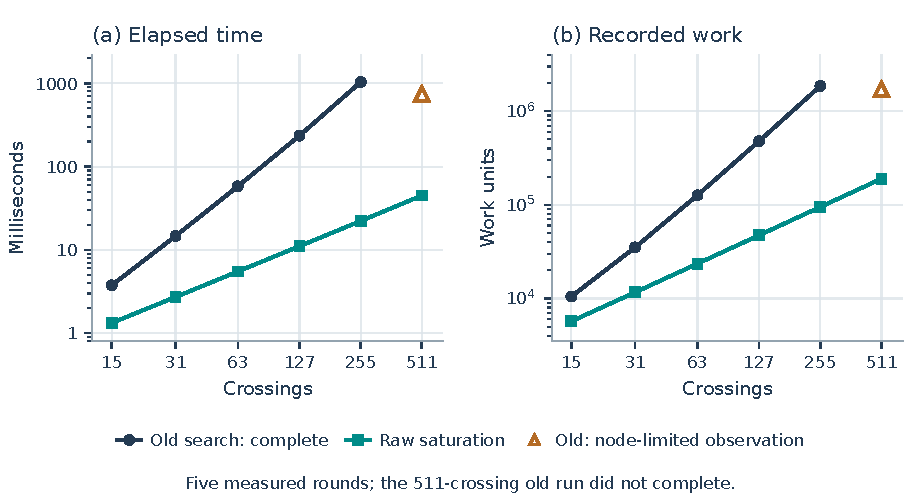
\includegraphics[width=\linewidth]{figures/raw_stage.pdf}
\caption{The complete group stage on elementary unknot closures.
Both source reconstruction and independent replay are included in
elapsed time. The marked old 511-crossing observation is node-censored.
These are mechanism controls, not a general hard-knot distribution.}
\label{fig:raw-stage}
\end{figure}

The maintained \texttt{unknot\_braid40} fixture improves from 22.536 to
3.387 ms in this isolated source-stage call, with paired ratio 6.625.
Other corpus cases show little benefit or regress. The paired ratios are
0.891 for \texttt{hard\_unknot\_8} and 0.912 for \texttt{monster}.
For \texttt{gordian}, the ratio is 1.010, too small to support a strong
elapsed-speed claim given the controls, and the exact work actually
increases. The source-stage benchmark cannot conclude knottedness when
group simplification fails: several nontrivial fixtures correctly remain
inconclusive in this positive-certificate stage.

\subsection{The failed-probe overhead and its correction}

The first candidate built a full support-incidence index before applying
the exact first-firing rejection test. On \texttt{gordian}, 137 of 139
queries failed this test, but 38,900 support incidences were nevertheless
materialized. The candidate used 986,374 work units against the
baseline's 789,805. Moving the guard before index construction reduces
this to 852,357, with only two indices and 32 materialized incidences.
The source audit confirms the same statuses and certificates as before.

This change removes most of the measured unnecessary index work, while
leaving an approximately 7.9\% work increase over baseline on this source.
The final work counts on \texttt{survivor-00} are 14,150 baseline versus
15,108 enabled; on \texttt{monster}, 5,357 versus 5,936. Both initial and
final records are supplied. It would be misleading to publish the large
algebraic-family speedup while omitting these failed-query costs.

\subsection{The surrounding recognizer changes the conclusion}

The full pipeline is tested on the 22 corpus fixtures with its normal
filters, a one-second total allowance, a 0.15-second local group
allowance, and the same remaining options for all arms. Every raw result
includes the terminal method and evidence, so an earlier filter's success
cannot be attributed to the new group producer. All conclusive outcomes
agree between arms. The full table is in
Appendix~\ref{app:full-tables}.

For example, \texttt{unknot\_braid40} is settled by the existing
genus-zero Seifert certificate before the group stage. Its full pipeline
times are about 0.21 ms in both arms, despite the large improvement when
the group stage is forced in isolation. The fixture \texttt{gst} is
rejected by the existing Alexander obstruction in about 1.3 ms, whereas
its positive-only group search stalls without a certificate. On
\texttt{gordian}, both pipelines reach the total time allowance and return
\texttt{UNKNOWN}; neither is credited with recognition.

For the survivor fixtures, enabled/full-pipeline paired ratios are mostly
slightly below one. The \texttt{monster} ratio is 0.903, corresponding
to medians 2.993 and 3.297 ms. Thus this corpus does not demonstrate a
broad improvement in full recognition speed. The new option remains
explicitly opt-in. Its supported benefit is complete raw reachability
and substantial improvement on some source-stage workloads, with the
observed regressions retained for future scheduling research.

\subsection{Orbit membership: independent graph audit and paired timings}

The eleven focused tests pass.  An exhaustive audit covers all systems with at most two interval generators
on universes of size at most five, up to input-generator order: $7{,}398$
indices across both merger rules and $34{,}026$ literal point checks.
The random audit prepares indices for $3{,}200$ random
interval relations under both maintained merger rules, giving $6{,}400$
checked indices and $208{,}000$ literal minimum comparisons.  A union-find
oracle explicitly expands only these bounded test inputs.  It also checks
$64{,}000$ sampled pair queries and all selected representatives, and all six
trace event types occur. The exhaustive and random tests also check the
complete canonical minimum interval set, sorted selection and ranks against
the literal graph. Two deliberately different valid traces establish
the distinction between canonical minimum labels and emission ordinals.

The geometric audit uses $67$ supplied normal vectors: parallel meridians
in one through ten tetrahedra and compatible mixtures of an interior
vertex sphere, a boundary vertex disc, and a one-sided M\"obius band in a
four-tetrahedron solid torus.  Both surface and boundary arc graphs are
tested under both merger rules, giving $268$ indices and another $73{,}528$
literal minimum comparisons.  These checks use the maintained exact
normal-coordinate adapter, with no native topology package required.
Separate tests cover $16{,}000$--$20{,}000$-bit endpoints, malformed and
unfinished proofs, source rebinding, caller mutation, disabled producer
entry points, and cancellation through false-valued callable objects.  A
separate exact fixture has $512$ disjoint minimum intervals and a $4{,}107$-bit
universe; its component count has $4{,}106$ bits, and the predicted $g=512$
interval bound is attained without enumerating components.

The portable paired benchmark has ten workloads, five shuffled arms,
one excluded warmup and seven measured rounds.  Single-query cases are
batched three times.  This gives $490$ measured complete arm calls and
$70$ warmup calls.  The compiled arm includes discovery, independent
verification, compilation and all requested comparisons.  The comparison
baseline shares the initial count and uses exact connected and singleton
shortcuts; only unresolved comparisons require augmented count schedules.
The original two-count API and identical controls are retained as separate
arms.  Every answer is compared outside the timer.

\begin{table}[htbp]
\centering
\caption{Complete repeated-membership workloads on supplied interval relations.
Discovery, independent verification, construction, and all queries are timed.
Times are milliseconds; ratios are paired medians.}
\label{tab:orbit-membership}
% Generated by generate_artifacts.py; edit the source JSON or generator.
\begingroup
\small
\setlength{\tabcolsep}{5pt}
\renewcommand{\arraystretch}{1.12}
\begin{tabular}{@{}p{6.5cm}rrrr@{}}
\toprule
Supplied relation & $q$ & Shared (ms) & Compiled (ms) & Ratio \\
\midrule
Meridian, $t=8$, scale $2^{512}+1$ & 1 & 2.845 & 2.993 & 0.925 \\
Meridian, $t=8$, scale $2^{512}+1$ & 8 & 12.880 & 2.852 & 4.582 \\
Meridian, $t=8$, scale $2^{512}+1$ & 32 & 46.957 & 2.996 & 15.629 \\
Meridian, $t=24$, scale $2^{128}+1$ & 1 & 25.157 & 20.437 & 1.224 \\
Meridian, $t=24$, scale $2^{128}+1$ & 8 & 111.298 & 20.308 & 5.502 \\
Meridian, $t=24$, scale $2^{128}+1$ & 32 & 422.509 & 20.539 & 20.686 \\
Primitive meridian, $t=8$ & 32 & 1.231 & 2.546 & 0.461 \\
M\"obius band, scale $2^{1024}+1$ & 32 & 1.540 & 0.321 & 4.447 \\
Four-tetrahedron compatible mixture & 32 & 29.527 & 2.124 & 13.915 \\
64-pair periodic chain & 32 & 14.182 & 1.629 & 8.757 \\
\bottomrule
\end{tabular}
\endgroup

\end{table}


\begin{figure}[htbp]
\centering
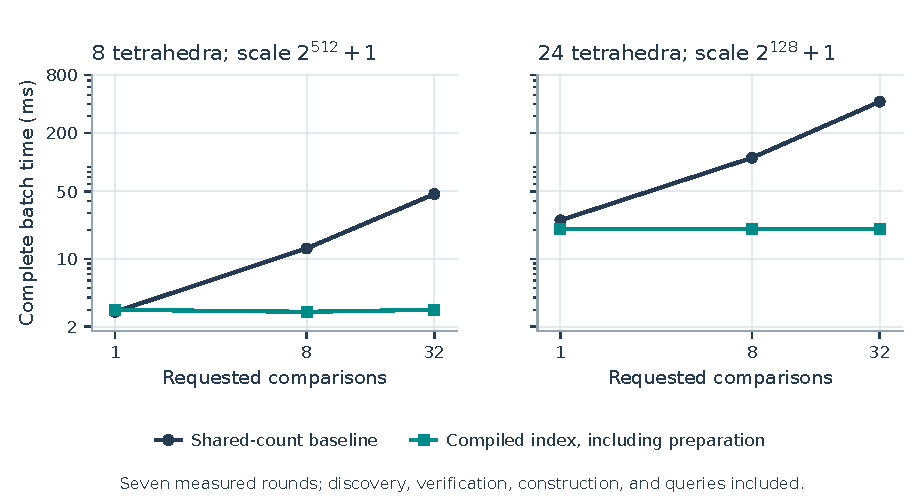
\includegraphics[width=\linewidth]{figures/orbit_queries.pdf}
\caption{Total membership-batch time as the number of requested comparisons
increases. Both compiled curves include preparation. No asymptotic law is
estimated from these finite observations.}
\label{fig:orbit-queries}
\end{figure}

Times are separate medians; the ratio is the median of paired ratios and
need not equal their quotient.  For the eight-tetrahedron source, the full
trace has $128$ events but the query program has $13$ point steps.  For
$24$ tetrahedra these figures are $832$ and $29$.  The periodic chain
compiles $65$ trace events to two point steps.  These are exact reductions
in work representation, independent of timer variation.

The primitive meridian is a necessary control: its first count proves the
relation connected, so the shared baseline answers all comparisons
immediately and is faster than index preparation.  The single-query
eight-tetrahedron case likewise shows no improvement.  Across all cases,
identical shared-control ratios range from $0.959$ to $1.040$, and
identical compiled-control ratios range from $0.969$ to $1.050$.  Thus the
large repeated-query effects are supported, while small percentage
differences should not be overinterpreted.

Raw records, inputs, query points, expected answers, reduction counts,
all shuffled arm orders and timings, and pre/post source hashes are in
\path{results/orbit_index.json}.  Audit evidence is in
\path{results/orbit_index_audit.json}; the portable drivers are in
\path{orbit_index_research/}.  Earlier prototype timings are not mixed into this table. Normal triangulation creation,
vector construction and conversion to interval relations are outside every
timer.  These results measure repeated queries on a supplied interval system,
not complete normal-surface calls or unknot-recognition runtime.
\subsection{Prepared canonical rank and selection}

The additional lookup experiment uses the sharp family of disjoint paired
blocks.  A supplied deterministic right-to-left trace is independently
verified before any query is timed.  The canonical minimum intervals and
every queried answer are checked against the direct block formulas, including
the conversion between emission ordinal and increasing-minimum rank.  Both
selection arms request the same original representatives on the same prepared
index; their numerical ordinal arguments differ because the orders differ.

Each measured call contains $512$ lookups, batched three times.  There are
seven shuffled measured rounds, one excluded warmup, and identical controls
for canonical rank and canonical selection.  Index construction is reported
separately and excluded from every lookup timer.  The original trace-ordinal
selection method reverses contractions; the canonical method searches the
compact minimum-interval union.

\begin{table}[htbp]
\centering
\caption{Prepared representative selection: 512 queries per call. Both selection
arms return the same source minima using their corresponding ordinals.
Preparation is excluded here and reported in the text. Times are milliseconds.}
\label{tab:orbit-rank}
% Generated by generate_artifacts.py; edit the source JSON or generator.
\begingroup
\small
\setlength{\tabcolsep}{5pt}
\renewcommand{\arraystretch}{1.12}
\begin{tabular}{@{}rrrrrr@{}}
\toprule
\shortstack{Minimum\\intervals} & \shortstack{Endpoint\\bits} & \shortstack{Emission\\(ms)} & \shortstack{Canonical\\(ms)} & Ratio & \shortstack{Rank\\(ms)} \\
\midrule
1 & 130 & 0.218 & 0.123 & 1.756 & 0.154 \\
16 & 134 & 0.794 & 0.138 & 5.922 & 0.168 \\
128 & 4105 & 7.600 & 0.327 & 23.791 & 0.348 \\
512 & 4107 & 29.732 & 0.365 & 81.511 & 0.408 \\
\bottomrule
\end{tabular}
\endgroup

\end{table}


All times concern a complete $512$-query call.  Preparation took respectively
$0.101$, $0.863$, $37.003$ and $557.962$ milliseconds in separately recorded
single observations.  Thus the submillisecond prepared lookup times do not
describe construction of the index.  Identical canonical-selection control
ratios range from $1.007$ to $1.034$, and rank-control ratios from $0.977$ to
$1.026$.  The final case has $512(2^{4096}+3)$ components while storing just
$512$ minimum intervals.  The bit-complexity conclusion is logarithmic in
the number of stored intervals, with binary-integer and output costs charged;
the finite timings are not a constant-time claim.

Full inputs, queried canonical ranks and corresponding emission ordinals,
analytic expected minima, source hashes, certificate hashes and all raw
samples are retained in \path{results/orbit_rank_select.json}.  The standalone
driver is \path{orbit_index_research/rank_select.py}.  This experiment measures
prepared representative lookups, separately from the preceding complete
membership-batch benchmark and from all unknot-recognition work.


\subsection{What these measurements support}

The strongest conclusions combine mathematical proofs with exact
representation or work counts: all raw orders reduce to a source closure
query; repeated component requests reuse one checked trace; minimum
representatives occupy at most the recorded number of static gaps.
Large local elapsed improvements are consistent with those mechanisms.
The same evidence rejects a claim that every diagram, every query count,
or the complete recognizer necessarily becomes faster.

The recent ReAPR study is relevant to the next empirical comparison:
its authors report success on a much larger public collection of unknot
diagrams, while treating general effectiveness as an open mathematical
question~\cite{reapr}. That study uses different methods and hardware.
We have not run its full corpus or its implementation here, so no
cross-paper speed ranking is made. A future complete-recognizer study
should include those inputs and comparable certified diagram
simplification strategies, alongside adversarial compressed presentations.

\section{A conditional route to quasi-polynomial recognition}
\label{sec:research-agenda}

The two results remove identifiable costs from a larger recognition
argument. Theorem~\ref{thm:raw-closure-equivalence} replaces every successful
raw singleton epoch by one source query and one polynomial compilation;
its cost need not contain a factor exponential in the number of raw
batches. The orbit index replaces repeated schedule discovery for a fixed
interval relation by one verified preparation. Neither result chooses the
next presentation or surface. A global complexity theorem must account
for that choice, for the number of objects chosen, and for their full
encoded descriptions.

\subsection{Three obligations that cannot be interchanged}

\paragraph{Deterministic discovery.}
A short certificate with a polynomial verifier need not be findable in
polynomial time. For the algebraic operation studied here, this gap is
closed: a prescribed survivor set is decided by Horn closure, and every
one-element survivor set can be tried in polynomial time. For normal
surfaces and hierarchy moves, a comparable discovery theorem is still
required. Counting or interpreting the components of a supplied normal
surface, as in AHT~\cite{aht}, does not find a suitable compressing disc or
prove that a small candidate list contains one. Candidate generation must
charge rejected candidates and unsuccessful subsidiary searches, including
those that never produce a certificate.

\paragraph{Hierarchy depth and the generated frontier.}
After each certified normalization or geometric cut, another local query
may be cheap, yet exponentially many distinct states may arise. One needs
a bound on the total states generated, or a depth bound together with a
branching bound, or a proved bound on the frontier after justified
identifications. Memoization provides a bound only after the number of
keys is bounded. Likewise, a polynomial bound on the size of each boundary
pattern does not bound the number of admissible patterns. The hierarchy
outline in the announced algorithm~\cite{lackenby-talk} and the detailed
2026 development~\cite{lackenby-2026} motivate this separation; the latter
does not supply all costs needed for the proposed implementation.

\paragraph{Bit complexity, provenance, and attachments.}
The cost of a state includes its reachable word grammar, binary lengths,
source-slot records, triangulation or handle data, verified trace, and
the maps specifying how boundary and attachment marks are identified.
Generator provenance and the evidence connecting the native input to the
original diagram are part of the state. So are historical masks, retained
arena nodes, and caches when operations can inspect them. Polynomial
compressed word and curve primitives~\cite{schleimer,lackenby-curves}
apply to the size of their supplied encodings. They cannot be charged
against a smaller crossing count without a bound relating the two.

The following accounting statement makes a sufficient target precise. It
is conditional on a complete recognition scheme, rather than a claim that
the scheme described in its hypotheses has been constructed.

\begin{proposition}[A sufficient global accounting contract]
\label{prop:qp-accounting}
Let $n\ge2$ be the bit length of a knot diagram encoding. Suppose a
deterministic recognition scheme has sound decomposition rules, complete
successor generation, and correct terminal tests. Suppose its whole
execution processes at most $F(n)$ state occurrences, counting repeated
states unless their suppression is justified. At each occurrence assume:
\begin{enumerate}
\item all discovery work, including rejected candidates, takes at most
      $D(n)$ bit operations;
\item all representations and relevant historical data have at most
      $P(n)$ bits, and their construction, verification, terminal tests,
      and composition cost $P(n)^{O(1)}$;
\item at most $Q(n)$ prepared local queries are made, each costing
      $P(n)^{O(1)}$ bit operations.
\end{enumerate}
If the initial faithful conversion costs $n^{O(1)}$, then, for a fixed
constant $c$, the running time is bounded by
\[
 n^{O(1)}+F(n)\bigl(D(n)+(1+Q(n))P(n)^c\bigr).
 \tag{A}\label{eq:global-accounting}
\]
In particular, quasi-polynomial bounds on $F,D,P,Q$ imply a
quasi-polynomial bound for this complete scheme.
\end{proposition}

\begin{proof}
Charge preparation and verification when each state is processed, then
charge its discovery and queries. Summing these bounds gives
\eqref{eq:global-accounting}. A finite product or fixed power of functions
bounded by $\exp((\log n)^{O(1)})$ has the same form. Completeness and
correct terminal interpretation are hypotheses; the estimate does not
derive them from certificate verification.
\end{proof}

For example, depth $h(n)$ and at most $b(n)$ generated successors per
state give $F(n)\le\sum_{i=0}^{h(n)}b(n)^i$. Polynomial branching and
$h(n)=O((\log n)^2)$ yield $\exp(O((\log n)^3))$ states. To obtain the
stronger $\exp(O((\log n)^2))$ by this particular argument would require
$h(n)=O(\log n)$, or a compensating smaller frontier. If at most $W(n)$
state occurrences are processed at each level, the alternative bound is
$F(n)\le(h(n)+1)W(n)$. Each formulation still needs the independent
$D,P,Q$ bounds. A complete fallback preserves correctness but contributes
its own running time whenever reached; the new local results do not
remove that contribution.

\subsection{Algebraic questions after saturation}

\paragraph{1. Which source presentations admit small survivor sets?}
For a fixed source define
\[
 \kappa(R)=\min\{|S|:S\subseteq X,\ \cl(S)=X\}.
\]
Enumeration gives a concrete quasi-polynomial procedure for the query
$\kappa(R)\le O(\log n)$ on polynomially encoded sources. The next study
should identify presentation classes with a proved small value, together
with a terminal method for their residual presentations. Reducing to a
small alphabet alone is not a recognition algorithm. General uniquely
restricted matching optimization has hardness results~\cite{golumbic};
whether useful parameterized structure survives the source-word
restrictions is a separate question. Any proposed improvement should
state its parameter and compare against the explicit
$\binom rk(r+m+I)$ enumeration bound.

This question must distinguish original meridians from transformed
generators. On standard unreduced crossing words, the implications recover
the familiar Wirtinger propagation mechanism~\cite{wirtinger}. When
crossing labels coincide, freely reducing those words can introduce
additional implications; ordinary diagrammatic coloring is then not
automatically identical to source closure. After Whitehead or other
verified presentation transformations, current generators also need not
be meridians. Corollary~4.3 of~\cite{incompatibility} supplies unknot
diagrams with arbitrarily large diagrammatic Wirtinger number. Thus a
fixed-diagram bounded-seed completeness conjecture for ordinary coloring
is already false. A useful new theorem must specify the permitted
transformations and charge their discovery.

\paragraph{2. Can cancellation boundaries be controlled?}
The example $xy,xy^2$ shows that a single free-reduction boundary can
enable eliminations absent from the original closure. A precise next
problem is to parameterize the interactions across such boundaries:
for instance by a stated bound on the number of participating source
factors or on an explicitly defined interaction graph. The desired
theorem would construct a finite successor list, bound its total encoded
size, and prove that some listed successor preserves a successful
continuation. Merely bounding the number of letters cancelled in an
expanded word would be unsuitable for highly compressed inputs.
Counterexample families should force cancellation across many shared
grammar subwords, so that a proposed parameter cannot hide an exponential
number of distinct contexts.

\paragraph{3. Which witness choices preserve later search behavior?}
Same-donor rematching preserves the induced map in the free group; closure
over all source rows may choose another donor set and need not preserve
that map. Can one optimize a closure witness for compiled size, attachment
description, or the next verified move without enumerating exponentially
many donor sets? A first falsifiable target is an efficiently computable
cost model for a restricted source class, with either a proved
approximation bound or a counterexample to greedy choice. Experiments
must compare semantic endpoints when donor sets agree, and complete
subsequent search outcomes when they differ. Equality of immediate ranks
does not establish interchangeability of these states. Classical matching
acyclicity and Horn propagation~\cite{kozen,dowling} remain the underlying
tools, rather than additional novelty claims.

\paragraph{4. Is there a potential controlling successive normalized epochs?}
The removed raw-phase factor should now be replaced by an explicit measure
of the transformations that remain. A promising theorem would associate
each normalized state with a potential and show a decrease, a bounded
number of neutral moves, or a balanced decomposition along every required
branch. The potential must account for encoded grammar complexity as well
as generator count: long sequences of rank-preserving transformations are
not ruled out by rank reduction. Record proposed potentials on adversarial
families and actively search for increasing cycles before using them in a
depth argument. A bound observed on successful examples is not a bound on
the failed branches required by deterministic recognition.

\subsection{Geometric representations and complete discovery}

\paragraph{5. Can the prepared point map be accelerated further?}
The present index stores the entire minimum set as at most $g$ ordinary
intervals and answers canonical minimum rank and selection in
$O(B\log(g+2))$ bit work. An arbitrary point query still follows the
contraction and truncation program; its stated bound is
$O(sB^2\log(k+2))$. These are different query problems. A concrete next
target is near-linear preparation in the stored trace size, followed by
polylogarithmic dependence on $s$ for point transport, with binary
arithmetic charged. Test whether balanced composition of partial affine,
reflection, and remainder maps produces a controlled representation, or
whether its number of pieces necessarily grows rapidly. The compactness
of the minimum set alone does not bound this composition. Existing
compressed tracing histories~\cite{erickson-nayyeri} are essential prior
art for this question.

\paragraph{6. Which attachment descriptions stay compact under cutting?}
Minimum representatives identify components of one fixed source relation.
They neither identify components across different triangulations nor
encode arbitrary permutations of attachment points. Choose an explicit
attachment language---for example, ordered marked intervals with specified
partial isometries and source charts---and prove closure of that language
under each proposed cut, gluing, and simplification. The measurable target
is a bound on chart count, map size, coordinate bits, and provenance length
after a sequence of operations. A counterexample with exponentially many
required chart pieces would refute that representation choice even if all
individual component queries remain polynomial. Signed variants must
transport the established geometric orientation data; an interval
reflection by itself is not an orientation character of a surface.

\paragraph{7. What makes a useful surface deterministically discoverable?}
The next hierarchy implementation should specify one exact move and its
input contract, then prove both a complete candidate description and a
producer with an encoded running-time bound. This is preferable to
assuming an unspecified oracle for a useful normal surface. Separate the
number of surface candidates, the weight bits of each, and the boundary
patterns created by cutting. AHT and the new index handle supplied
component data; the curve algorithms can handle supplied compressed curves
\cite{aht,lackenby-curves}. The missing theorem must explain why the
necessary supplied objects can be found within the budget. The 2026
hierarchy preprint~\cite{lackenby-2026} gives a serious source of structural
lemmas, but each imported statement must retain its hypotheses and cost
parameters.

\paragraph{8. Can equivalent marked frontiers be recognized and counted?}
A frontier compression theorem needs an equivalence relation preserving
all permitted continuations, a procedure to recognize that equivalence,
and a bound on the number of resulting classes. Equal component counts,
equal lists of minimum ranks, or isomorphic unmarked graphs need not
preserve attachment maps or peripheral information. Start with a restricted
surface class and a fixed attachment language from Question~6. Construct
pairs with identical coarse summaries but different marked behavior; these
are direct tests of any proposed state key. Only after such distinctions
are resolved can canonicalization justify a smaller $W(n)$ in the global
contract.

\paragraph{9. Can marked component data be returned without listing components?}
The most direct next geometric extension is to associate the maintained
weighted terminal runs with canonical minimum keys. Given one marked
point, return its component's Euler characteristic, boundary information,
or complete normal coordinate vector, using compressed weight transport.
The target is preparation polynomial in the source trace and requested
weight channels, followed by queries that depend on the encoded answer
size. The minimum-set interval bound does not automatically bound the
number of weight changes within those intervals. Prove an additional
bound on the joint representation, or exhibit a family in which the
chosen weight language requires too many pieces. The signed-cover
corollary supplies path parity, provided that the geometric character
has already been certified; it does not replace this weighted analysis.

\paragraph{10. Which proof obligations can be mechanically formalized first?}
A focused formalization should begin with the positive-pivot matching
injection, the same-donor free-group homomorphism argument, and the
orbit minimum-set invariant. Each has a small mathematical interface and
an independent finite oracle already available for examples. A second
stage should prove refinement from immutable grammar masks and the
queue invariant to the mathematical closure, and from the six verified
interval operations to the retained transport program. The distinction
between equality of raw strings and equality in a free group must appear
in the formal statement. No machine-checked proof is included in this
delivery: the supplied proofs are mathematical manuscripts, and the
independent certificate replayers and tests remain software evidence.

\subsection{An adversarial validation and integration programme}

The next experiments should test explicit claims and expose their limits.
They should retain the pinned baseline and independently verified outputs
used in this continuation~\cite{repo}. Three complementary designs would
make progress assessable.

\paragraph{Algebraic stress tests.}
Extend the finite matrix audit with structured unique-matching families,
bad pivot orders, repeated donor roots, and entries of large binary size.
For word-level tests vary signs independently of absolute incidence,
include empty slots and sparse generator names, and require same-donor
flattening to preserve every freely reduced generator image and residual
relator. Include presentations in which one normalization changes closure,
and knot families built from the Wirtinger obstruction examples. Record
closure work, compiled nodes, retained historical storage, normalization
boundaries, and all explored branches separately. The matrix checks
support implementation correctness; they do not replace the proof or
model the distribution of knot diagrams.

\paragraph{Orbit and attachment stress tests.}
Vary endpoint bit length independently of pairing count, trace length,
gap count, and query count. Combine reflections, periodic carriers, and
separated static gaps; compare different valid traces for identical
minimum maps and canonical order. Test huge component counts with few
minimum intervals, as well as families attaining the interval bound.
Cross-check small cases by explicit union--find and large structured cases
by independent formulas. For performance, compare the same requested
representatives and include a baseline sharing the original orbit count.
Report verification and preparation separately from prepared queries and
also as a complete workload, so the break-even query count is visible.

\paragraph{End-to-end and negative tests.}
Use held-out diagram families, verified diagram transformations, and
nontrivial knots, rather than only successful local certificates. Report
success, certified rejection, and resource exhaustion separately.
Mutations should target source bindings, donor reuse, ranks outside the
minimum set, attachment maps, incomplete traces, and arithmetic limits.
Record actual encoded sizes, peak retained memory, source hashes, raw
timings, and discovered-state counts. No finite timing fit establishes
the exponent in an asymptotic theorem; the useful outcome is either a
counterexample to a proposed bound or data identifying which obligation
in~\eqref{eq:global-accounting} dominates.

The resulting milestones are concrete: first, an exact and measured
normalization-boundary model; second, a closed language of marked
geometric states with composable provenance; third, a complete candidate
producer for a specified hierarchy move; and finally a proved frontier or
depth bound. The present saturation and indexing results supply reliable
local operations for that programme. The remaining global hypotheses are
research problems, not consequences of those local operations.

\appendix
\section{Archive layout and reproducibility}
\label{app:reproducibility}

The archive is a reviewable continuation against the pinned source,
not a remote repository update. It contains the complete article and
its figures, the modified \texttt{fast} source tree, an executable
baseline snapshot for comparisons, the required reference modules,
raw experimental evidence, and an integration patch. The existing
project license is retained with the source.

\subsection{File map}

\begin{description}[style=nextline,leftmargin=0pt,labelsep=0pt,labelwidth=0pt]
\item[\path{article/}]
  The main source \path{compiled_certificates.tex}, all included
  sections, the rendered PDF, generated tables, figure PDFs and PNGs,
  and \path{generate_artifacts.py}. No network access is required to
  rebuild the manuscript from the included sources.
\item[\path{fast/fastunknot/}]
  The full current runtime snapshot. The new modules are
  \path{raw_saturation.py} and \path{orbit_index.py}. Four existing
  files gain the optional group hook: \path{compressed_search.py},
  \path{group_certificate.py}, \path{recognize.py}, and
  \path{__main__.py}.
\item[\path{fast/tests/}]
  The maintained suite, including the three new test files
  \path{test_raw_saturation.py},
  \path{test_raw_saturation_integration.py}, and
  \path{test_orbit_index.py}.
\item[\path{fast/raw_saturation_research/}]
  The independent matrix/signed-word audit, four-mode benchmark,
  summary generator, and frozen initial-candidate snapshot. The
  initial snapshot explains the failed-probe optimization; its
  measurements are explicitly separated from the final candidate.
\item[\path{fast/orbit_index_research/}]
  The graph audit, complete membership benchmark, prepared rank/select
  benchmark, API documentation, and mathematical research notes.
\item[\path{fast/results/}]
  Exact inputs, raw timing samples, all outcomes, checked source hashes,
  logs, per-arm journals, and generated summaries. Only the completed
  final records supply headline values.
\item[\path{baseline/fast/} and \path{baseline/reports/}]
  The pinned runtime/test snapshot and its required reference modules.
  These support the paired group comparisons and the baseline suite
  without downloading the upstream repository.
\item[\path{reports/}]
  The exact reference Python modules from reports 24, 26, 28, and 45
  needed by existing tests. They are included because the maintained
  suite imports them from outside \texttt{fast}.
\item[\path{provenance/}]
  The Git-blob source manifest, archive-content hashes, environment
  record, baseline/final suite logs, and patch verification results.
\item[\path{integration.patch}]
  A source patch against the pinned repository paths, adding the two
  runtime modules, the optional hook, tests, and research drivers.
  The article and bulky experimental evidence are separately organized
  for repository placement.
\end{description}

The source manifest records the retrieval audit, including read-only
synthesis sources used during research. Those synthesis sources are not
all duplicated in the delivery. The archive-content manifest separately
identifies the files actually packaged. Baseline source bytes were checked
against their Git blob identifiers; current experimental source hashes
were checked before and after the measurements. The group source-hash
set excludes the unrelated orbit module, whose own evidence carries
complete separate hashes.

\subsection{Rebuilding and running the checks}

The runtime declares Python 3.10 or later and no mandatory package
dependencies. The recorded environment is Python 3.12.14, Regina 7.4.1,
NumPy 2.3.5, and Matplotlib 3.10.8. The full historical suite has tests
for optional native normal-surface functionality, so reproducing every
recorded test requires the supplied environment or the documented
Regina extra. The new saturation and orbit-index tests themselves use
the Python implementation and independent finite oracles.

From the archive's top directory, the principal commands are:
\begin{verbatim}
cd fast
python3 -B -m unittest discover -s tests -q
python3 -B raw_saturation_research/audit_epoch.py
python3 -B raw_saturation_research/benchmark.py \
  --mode audit --candidate-label final-preindex-guard \
  --output results/raw_saturation_audit.json
python3 -B raw_saturation_research/benchmark.py \
  --mode kernels --candidate-label final-preindex-guard \
  --output results/raw_saturation_kernels.json
python3 -B raw_saturation_research/benchmark.py \
  --mode stage --candidate-label final-preindex-guard \
  --output results/raw_saturation_stage.json
python3 -B raw_saturation_research/benchmark.py \
  --mode pipeline --candidate-label final-preindex-guard \
  --output results/raw_saturation_pipeline.json
python3 -B raw_saturation_research/summarize.py
python3 -B orbit_index_research/audit.py
python3 -B orbit_index_research/benchmark.py --rounds 7
python3 -B orbit_index_research/rank_select.py --rounds 7
\end{verbatim}
The group benchmark's default baseline location is
\path{../baseline/fast}. A separate checkout can be supplied with
\texttt{--baseline}. These commands replace the correspondingly named
result files; preserve the delivered records in another directory before
an independent replication. Run timing experiments without simultaneous
CPU-intensive tests. Random call order and controls reduce some timer
effects but do not turn a shared machine into an isolated laboratory.

From the archive's top directory, regenerate the numerical artifacts and PDF:
\begin{verbatim}
cd article
python3 generate_artifacts.py --results ../fast/results
latexmk -pdf -interaction=nonstopmode -halt-on-error \
  compiled_certificates.tex
\end{verbatim}
Two or more ordinary \texttt{pdflatex} passes can replace
\texttt{latexmk}. The preamble uses common TeX Live packages, with no
shell-escape requirement or external bibliography processor. The provided
PDF was rendered to page images and inspected for clipping, table
overflow, unresolved references, and figure readability.

\subsection{Review and integration order}

First review the mathematical theorem statements together with their
counterexamples. Next review the two runtime modules and the four small
option-plumbing changes. Apply the source patch to a clean checkout of
the pinned commit, or reconcile it manually with a newer upstream
revision; test commands should run from the \texttt{fast} directory.
The patch does not assign a new report number or overwrite the existing
synthesis manuscript. The standalone article can be moved to the
maintainer's chosen research location with all its included files.

The raw producer requires no certificate-verifier change. Its final
source proofs were checked by the old and current replayers. The orbit
index's documented factory independently verifies the entire supplied
trace, but its query arithmetic is an additional trusted implementation.
Its immutability contract concerns factory-created objects; manually
constructing private Python dataclass fields is outside that interface.
These are distinct trust boundaries and should remain distinct during
integration.

No general quasi-polynomial flag is enabled. The existing recognizer's
worst-case statement remains appropriate. The finite audit supplies no
claim that all possible mutants, diagrams, or interval systems have been
tested. The proofs establish the local statements; the recorded evidence
checks their implementation and the observed performance on specified
inputs.

\section{Complete group benchmark tables}
\label{app:full-tables}

In the following tables, U denotes \texttt{UNKNOT}, K denotes
\texttt{KNOTTED}, I denotes a positive-only group-stage
\texttt{INCONCLUSIVE}, and ? denotes full-pipeline \texttt{UNKNOWN}.
Times are milliseconds. A dash in a completion-time or ratio column
indicates an unavailable completed comparison; it is not zero. Observed
elapsed-time columns are populated only for unresolved arms.
Exact observed times and the reason for each unfinished call are retained
in the JSON and per-arm journals. All conclusive paired statuses agree.

\subsection{Group stage: reconstruction, search, and independent replay}

% Generated by generate_artifacts.py. This is a longtable, not a float.
\begingroup
\small
\setlength{\tabcolsep}{3pt}
\setlength{\LTcapwidth}{\linewidth}
\renewcommand{\arraystretch}{1.08}
\begin{longtable}{@{}>{\raggedright\arraybackslash}p{3.45cm}rrrrrrc@{}}
\caption{Full group-stage benchmark: all 28 inputs.}\label{tab:raw-stage-full}\\
\toprule
Input & $n$ & \shortstack{Old\\complete} & \shortstack{New\\complete} & \shortstack{Old\\observed} & \shortstack{New\\observed} & Ratio & \shortstack{Old/new\\status} \\
\midrule
\endfirsthead
\toprule
Input & $n$ & \shortstack{Old\\complete} & \shortstack{New\\complete} & \shortstack{Old\\observed} & \shortstack{New\\observed} & Ratio & \shortstack{Old/new\\status} \\
\midrule
\endhead
\midrule
\multicolumn{8}{r}{\footnotesize Continued on the next page.}\\
\endfoot
\bottomrule
\multicolumn{8}{@{}p{\linewidth}@{}}{\footnotesize All times are milliseconds. Completion medians and paired ratios are copied from the recorded JSON summaries. An unresolved arm has -- for completion time and no completion ratio; only then is its observed elapsed median shown. U = \texttt{UNKNOT}, K = \texttt{KNOTTED}, I = \texttt{INCONCLUSIVE}, ? = \texttt{UNKNOWN}. All measured outcomes for each arm agree within every row in this data set.}\\
\endlastfoot
\texttt{circle-\allowbreak 15} & 15 & 3.751 & 1.325 & -- & -- & 2.814 & U/U \\
\texttt{circle-\allowbreak 31} & 31 & 14.620 & 2.712 & -- & -- & 5.311 & U/U \\
\texttt{circle-\allowbreak 63} & 63 & 57.965 & 5.498 & -- & -- & 10.290 & U/U \\
\texttt{circle-\allowbreak 127} & 127 & 234.973 & 11.059 & -- & -- & 20.393 & U/U \\
\texttt{circle-\allowbreak 255} & 255 & 1\,036.076 & 22.204 & -- & -- & 46.720 & U/U \\
\texttt{circle-\allowbreak 511} & 511 & -- & 44.922 & 742.769 & -- & -- & I/U \\
\texttt{survivor-\allowbreak 00} & 16 & 7.648 & 7.130 & -- & -- & 0.964 & U/U \\
\texttt{survivor-\allowbreak 01} & 15 & 5.662 & 5.912 & -- & -- & 0.949 & U/U \\
\texttt{survivor-\allowbreak 02} & 15 & 6.428 & 6.446 & -- & -- & 1.009 & U/U \\
\texttt{survivor-\allowbreak 03} & 13 & 4.507 & 4.494 & -- & -- & 0.992 & U/U \\
\texttt{survivor-\allowbreak 04} & 13 & 3.771 & 3.755 & -- & -- & 0.996 & U/U \\
\texttt{survivor-\allowbreak 05} & 13 & 8.321 & 8.387 & -- & -- & 1.018 & U/U \\
\texttt{survivor-\allowbreak 06} & 12 & 2.876 & 2.971 & -- & -- & 0.974 & U/U \\
\texttt{survivor-\allowbreak 07} & 12 & 8.693 & 8.791 & -- & -- & 0.985 & U/U \\
\texttt{survivor-\allowbreak 08} & 11 & 2.977 & 2.947 & -- & -- & 1.004 & U/U \\
\texttt{survivor-\allowbreak 09} & 11 & 3.055 & 3.015 & -- & -- & 0.985 & U/U \\
\texttt{survivor-\allowbreak 10} & 11 & 2.807 & 2.597 & -- & -- & 1.083 & U/U \\
\texttt{survivor-\allowbreak 11} & 11 & 2.668 & 2.685 & -- & -- & 0.981 & U/U \\
\texttt{trefoil} & 3 & -- & -- & 0.712 & 0.625 & -- & I/I \\
\texttt{conway} & 11 & -- & -- & 7.777 & 7.630 & -- & I/I \\
\texttt{kinoshita\_\allowbreak terasaka} & 11 & -- & -- & 12.983 & 12.896 & -- & I/I \\
\texttt{hard\_\allowbreak unknot\_\allowbreak 8} & 8 & 1.277 & 1.440 & -- & -- & 0.891 & U/U \\
\texttt{grid\_\allowbreak determinant\_\allowbreak one\_\allowbreak knot} & 10 & -- & -- & 2.450 & 2.493 & -- & I/I \\
\texttt{unknot\_\allowbreak braid40} & 40 & 22.536 & 3.387 & -- & -- & 6.625 & U/U \\
\texttt{stress\_\allowbreak braid5\_\allowbreak 36} & 36 & -- & -- & 68.986 & 76.205 & -- & I/I \\
\texttt{monster} & 10 & 2.095 & 2.202 & -- & -- & 0.912 & U/U \\
\texttt{gst} & 48 & -- & -- & 789.078 & 756.285 & -- & I/I \\
\texttt{gordian} & 141 & 393.890 & 380.828 & -- & -- & 1.010 & U/U \\
\end{longtable}
\endgroup


\subsection{Full recognizer with ordinary filters and fixed allowances}

% Generated by generate_artifacts.py. This is a longtable, not a float.
\begingroup
\small
\setlength{\tabcolsep}{3pt}
\setlength{\LTcapwidth}{\linewidth}
\renewcommand{\arraystretch}{1.08}
\begin{longtable}{@{}>{\raggedright\arraybackslash}p{3.45cm}rrrrrrc@{}}
\caption{All full-recognizer benchmark inputs.}\label{tab:raw-pipeline-full}\\
\toprule
Input & $n$ & \shortstack{Old\\complete} & \shortstack{New\\complete} & \shortstack{Old\\observed} & \shortstack{New\\observed} & Ratio & \shortstack{Old/new\\status} \\
\midrule
\endfirsthead
\toprule
Input & $n$ & \shortstack{Old\\complete} & \shortstack{New\\complete} & \shortstack{Old\\observed} & \shortstack{New\\observed} & Ratio & \shortstack{Old/new\\status} \\
\midrule
\endhead
\midrule
\multicolumn{8}{r}{\footnotesize Continued on the next page.}\\
\endfoot
\bottomrule
\multicolumn{8}{@{}p{\linewidth}@{}}{\footnotesize All times are milliseconds. Completion medians and paired ratios are copied from the recorded JSON summaries. An unresolved arm has -- for completion time and no completion ratio; only then is its observed elapsed median shown. U = \texttt{UNKNOT}, K = \texttt{KNOTTED}, I = \texttt{INCONCLUSIVE}, ? = \texttt{UNKNOWN}. All measured outcomes for each arm agree within every row in this data set.}\\
\endlastfoot
\texttt{survivor-\allowbreak 00} & 16 & 9.901 & 10.219 & -- & -- & 0.997 & U/U \\
\texttt{survivor-\allowbreak 01} & 15 & 7.899 & 8.089 & -- & -- & 0.980 & U/U \\
\texttt{survivor-\allowbreak 02} & 15 & 8.498 & 8.977 & -- & -- & 0.968 & U/U \\
\texttt{survivor-\allowbreak 03} & 13 & 6.067 & 6.183 & -- & -- & 0.980 & U/U \\
\texttt{survivor-\allowbreak 04} & 13 & 5.256 & 5.425 & -- & -- & 0.962 & U/U \\
\texttt{survivor-\allowbreak 05} & 13 & 10.436 & 10.756 & -- & -- & 0.971 & U/U \\
\texttt{survivor-\allowbreak 06} & 12 & 4.238 & 4.314 & -- & -- & 0.982 & U/U \\
\texttt{survivor-\allowbreak 07} & 12 & 11.189 & 11.394 & -- & -- & 0.982 & U/U \\
\texttt{survivor-\allowbreak 08} & 11 & 4.159 & 4.241 & -- & -- & 0.974 & U/U \\
\texttt{survivor-\allowbreak 09} & 11 & 4.279 & 4.423 & -- & -- & 0.979 & U/U \\
\texttt{survivor-\allowbreak 10} & 11 & 3.971 & 4.051 & -- & -- & 0.980 & U/U \\
\texttt{survivor-\allowbreak 11} & 11 & 3.960 & 3.960 & -- & -- & 1.001 & U/U \\
\texttt{trefoil} & 3 & 0.036 & 0.034 & -- & -- & 1.053 & K/K \\
\texttt{conway} & 11 & 0.645 & 0.645 & -- & -- & 0.960 & K/K \\
\texttt{kinoshita\_\allowbreak terasaka} & 11 & 0.599 & 0.631 & -- & -- & 1.027 & K/K \\
\texttt{hard\_\allowbreak unknot\_\allowbreak 8} & 8 & 1.427 & 1.496 & -- & -- & 0.954 & U/U \\
\texttt{grid\_\allowbreak determinant\_\allowbreak one\_\allowbreak knot} & 10 & 0.069 & 0.064 & -- & -- & 1.005 & K/K \\
\texttt{unknot\_\allowbreak braid40} & 40 & 0.213 & 0.211 & -- & -- & 1.011 & U/U \\
\texttt{stress\_\allowbreak braid5\_\allowbreak 36} & 36 & 0.628 & 0.630 & -- & -- & 0.973 & K/K \\
\texttt{monster} & 10 & 2.993 & 3.297 & -- & -- & 0.903 & U/U \\
\texttt{gst} & 48 & 1.336 & 1.312 & -- & -- & 0.989 & K/K \\
\texttt{gordian} & 141 & -- & -- & 1\,015.181 & 1\,020.367 & -- & ?/? \\
\end{longtable}
\endgroup


\begin{thebibliography}{99}
\raggedright
\addcontentsline{toc}{section}{References}

\bibitem{repo}
Vladimir Reshetnikov, \emph{ProveIt: Topology/UnknotRecognition}, source
commit \texttt{fdeb5b1a20b84b93cb150e0232031837bb7d30cb},
9 October 2026 UTC.
\href{https://github.com/VladimirReshetnikov/ProveIt/tree/fdeb5b1a20b84b93cb150e0232031837bb7d30cb/Topology/UnknotRecognition}{Pinned repository tree}.
In particular, the maintained \texttt{fast} implementation, tests,
research drivers, and accompanying \texttt{synthesis} sections.

\bibitem{aht}
Ian Agol, Joel Hass, and William Thurston,
\emph{The computational complexity of knot genus and spanning area},
Transactions of the American Mathematical Society \textbf{358}(9)
(2006), 3821--3850.
\href{https://arxiv.org/abs/math/0205057v2}{arXiv:math/0205057v2}.
The orbit-counting and weighted results are Theorems 12 and 16 in the
referenced preprint version.

\bibitem{lackenby-talk}
Marc Lackenby, \emph{Unknot recognition in quasi-polynomial time},
Oxford talk handout, March 2021.
\href{https://people.maths.ox.ac.uk/lackenby/quasipolynomial-talk-oxford-compressed.pdf}{Author's handout}.
The announced $2^{O((\log n)^3)}$ bound appears on slide 7;
the hierarchy-depth outline appears on slide 25.

\bibitem{lackenby-2026}
Marc Lackenby, \emph{Incompressible surfaces, hierarchies and unknot
recognition}, preprint, 25 July 2026.
\href{https://arxiv.org/abs/2607.23350v1}{arXiv:2607.23350v1}.
See Section 9 for the complexity discussion and Proposition 9.1.

\bibitem{lackenby-curves}
Marc Lackenby, \emph{Some fast algorithms for curves in surfaces},
Discrete \& Computational Geometry \textbf{76} (2026), 539--588.
\href{https://doi.org/10.1007/s00454-026-00845-7}{doi:10.1007/s00454-026-00845-7}.

\bibitem{schleimer}
Saul Schleimer, \emph{Polynomial-time word problems},
Commentarii Mathematici Helvetici \textbf{83}(4) (2008), 741--765.
\href{https://doi.org/10.4171/CMH/142}{doi:10.4171/CMH/142}.
\href{https://arxiv.org/abs/math/0608563}{arXiv:math/0608563}.

\bibitem{kozen}
D. Kozen, U. V. Vazirani, and V. V. Vazirani,
\emph{NC algorithms for comparability graphs, interval graphs, and
testing for unique perfect matching}, in Foundations of Software Technology and
Theoretical Computer Science, Lecture Notes in Computer Science
\textbf{206} (1985), 496--503.
\href{https://doi.org/10.1007/3-540-16042-6_28}{doi:10.1007/3-540-16042-6\_28}.
Expanded as \emph{NC Algorithms for Comparability Graphs, Interval Graphs,
and Unique Perfect Matchings}, Cornell TR 86-799 (1986).
\href{https://www.cs.cornell.edu/~kozen/Papers/comp.pdf}{Authors' manuscript}.
The source matching/acyclicity characterization is classical.

\bibitem{golumbic}
M. C. Golumbic, T. Hirst, and M. Lewenstein,
\emph{Uniquely restricted matchings}, Algorithmica \textbf{31}(2)
(2001), 139--154.
\href{https://doi.org/10.1007/s00453-001-0004-z}{doi:10.1007/s00453-001-0004-z}.

\bibitem{dowling}
William F. Dowling and Jean H. Gallier,
\emph{Linear-time algorithms for testing the satisfiability of
propositional Horn formulae}, Journal of Logic Programming
\textbf{1}(3) (1984), 267--284.
\href{https://doi.org/10.1016/0743-1066(84)90014-1}{doi:10.1016/0743-1066(84)90014-1}.
\href{https://www.seas.upenn.edu/~cis5110/Dowling-Gallier-Horn-sat.pdf}{Authors' article copy}.

\bibitem{wirtinger}
Ryan Blair, Alexandra Kjuchukova, Roman Velazquez, and Paul Villanueva,
\emph{Wirtinger systems of generators of knot groups},
Communications in Analysis and Geometry \textbf{28}(2) (2020), 243--262.
\href{https://doi.org/10.4310/CAG.2020.v28.n2.a2}{doi:10.4310/CAG.2020.v28.n2.a2}.
\href{https://arxiv.org/abs/1705.03108}{arXiv:1705.03108}.

\bibitem{incompatibility}
Ryan Blair, Alexandra Kjuchukova, and Makoto Ozawa,
\emph{The incompatibility of crossing number and bridge number for knot
diagrams}, Discrete Mathematics \textbf{342}(7) (2019), 1966--1978.
\href{https://doi.org/10.1016/j.disc.2019.03.013}{doi:10.1016/j.disc.2019.03.013}.
\href{https://arxiv.org/abs/1710.11327}{arXiv:1710.11327}.

\bibitem{erickson-nayyeri}
Jeff Erickson and Amir Nayyeri,
\emph{Tracing compressed curves in triangulated surfaces},
Discrete \& Computational Geometry \textbf{49}(4) (2013), 823--863.
\href{https://jeffe.cs.illinois.edu/pubs/pdf/tracing.pdf}{Authors' manuscript}.
Section 3.3 discusses the compressed tracing history.

\bibitem{papakyriakopoulos}
C. D. Papakyriakopoulos,
\emph{On Dehn's lemma and the asphericity of knots},
Proceedings of the National Academy of Sciences of the United States
of America \textbf{43}(1) (1957), 169--172.
\href{https://doi.org/10.1073/pnas.43.1.169}{doi:10.1073/pnas.43.1.169}.
Theorem 3(i) states the free-cyclic knot-group characterization of the
unknot. The longer proof appears under the same title in Annals of
Mathematics \textbf{66}(1) (1957), 1--26.

\bibitem{reapr}
Jason Cantarella, Henrik Schumacher, and Clayton Shonkwiler,
\emph{Hard unknots are often easy from a different perspective},
preprint, version 3, October 2026.
\href{https://arxiv.org/abs/2607.28772v3}{arXiv:2607.28772v3}.
The associated test sets are available at
\href{https://doi.org/10.5061/dryad.vx0k6dk6v}{doi:10.5061/dryad.vx0k6dk6v}.

\end{thebibliography}

\end{document}
